\documentclass[twoside]{book}

% Packages required by doxygen
\usepackage{fixltx2e}
\usepackage{calc}
\usepackage{doxygen}
\usepackage[export]{adjustbox} % also loads graphicx
\usepackage{graphicx}
\usepackage[utf8]{inputenc}
\usepackage{makeidx}
\usepackage{multicol}
\usepackage{multirow}
\PassOptionsToPackage{warn}{textcomp}
\usepackage{textcomp}
\usepackage[nointegrals]{wasysym}
\usepackage[table]{xcolor}

% Font selection
\usepackage[T1]{fontenc}
\usepackage[scaled=.90]{helvet}
\usepackage{courier}
\usepackage{amssymb}
\usepackage{sectsty}
\renewcommand{\familydefault}{\sfdefault}
\allsectionsfont{%
  \fontseries{bc}\selectfont%
  \color{darkgray}%
}
\renewcommand{\DoxyLabelFont}{%
  \fontseries{bc}\selectfont%
  \color{darkgray}%
}
\newcommand{\+}{\discretionary{\mbox{\scriptsize$\hookleftarrow$}}{}{}}

% Page & text layout
\usepackage{geometry}
\geometry{%
  a4paper,%
  top=2.5cm,%
  bottom=2.5cm,%
  left=2.5cm,%
  right=2.5cm%
}
\tolerance=750
\hfuzz=15pt
\hbadness=750
\setlength{\emergencystretch}{15pt}
\setlength{\parindent}{0cm}
\setlength{\parskip}{3ex plus 2ex minus 2ex}
\makeatletter
\renewcommand{\paragraph}{%
  \@startsection{paragraph}{4}{0ex}{-1.0ex}{1.0ex}{%
    \normalfont\normalsize\bfseries\SS@parafont%
  }%
}
\renewcommand{\subparagraph}{%
  \@startsection{subparagraph}{5}{0ex}{-1.0ex}{1.0ex}{%
    \normalfont\normalsize\bfseries\SS@subparafont%
  }%
}
\makeatother

% Headers & footers
\usepackage{fancyhdr}
\pagestyle{fancyplain}
\fancyhead[LE]{\fancyplain{}{\bfseries\thepage}}
\fancyhead[CE]{\fancyplain{}{}}
\fancyhead[RE]{\fancyplain{}{\bfseries\leftmark}}
\fancyhead[LO]{\fancyplain{}{\bfseries\rightmark}}
\fancyhead[CO]{\fancyplain{}{}}
\fancyhead[RO]{\fancyplain{}{\bfseries\thepage}}
\fancyfoot[LE]{\fancyplain{}{}}
\fancyfoot[CE]{\fancyplain{}{}}
\fancyfoot[RE]{\fancyplain{}{\bfseries\scriptsize Generated by Doxygen }}
\fancyfoot[LO]{\fancyplain{}{\bfseries\scriptsize Generated by Doxygen }}
\fancyfoot[CO]{\fancyplain{}{}}
\fancyfoot[RO]{\fancyplain{}{}}
\renewcommand{\footrulewidth}{0.4pt}
\renewcommand{\chaptermark}[1]{%
  \markboth{#1}{}%
}
\renewcommand{\sectionmark}[1]{%
  \markright{\thesection\ #1}%
}

% Indices & bibliography
\usepackage{natbib}
\usepackage[titles]{tocloft}
\setcounter{tocdepth}{3}
\setcounter{secnumdepth}{5}
\makeindex

% Hyperlinks (required, but should be loaded last)
\usepackage{ifpdf}
\ifpdf
  \usepackage[pdftex,pagebackref=true]{hyperref}
\else
  \usepackage[ps2pdf,pagebackref=true]{hyperref}
\fi
\hypersetup{%
  colorlinks=true,%
  linkcolor=blue,%
  citecolor=blue,%
  unicode%
}

% Custom commands
\newcommand{\clearemptydoublepage}{%
  \newpage{\pagestyle{empty}\cleardoublepage}%
}

\usepackage{caption}
\captionsetup{labelsep=space,justification=centering,font={bf},singlelinecheck=off,skip=4pt,position=top}

%===== C O N T E N T S =====

\begin{document}

% Titlepage & ToC
\hypersetup{pageanchor=false,
             bookmarksnumbered=true,
             pdfencoding=unicode
            }
\pagenumbering{alph}
\begin{titlepage}
\vspace*{7cm}
\begin{center}%
{\Large Geus }\\
\vspace*{1cm}
{\large Generated by Doxygen 1.8.13}\\
\end{center}
\end{titlepage}
\clearemptydoublepage
\pagenumbering{roman}
\tableofcontents
\clearemptydoublepage
\pagenumbering{arabic}
\hypersetup{pageanchor=true}

%--- Begin generated contents ---
\chapter{R\+E\+A\+D\+ME}
\label{md_README}
\Hypertarget{md_README}
A very simple Shoot em Up game created as a midterm project of the B\+I-\/\+P\+A2 subject at C\+TU F\+IT in Prague.

{\bfseries Installation}


\begin{DoxyItemize}
\item download the project somewhere using \begin{DoxyVerb}  git clone https://github.com/Tajnymag/geus.git
\end{DoxyVerb}

\item step into the directory and run the provided Makefile \begin{DoxyVerb}  cd geus;
  make
\end{DoxyVerb}

\item you should be able to run the game by issuing \begin{DoxyVerb}  make run
\end{DoxyVerb}

\end{DoxyItemize}

{\bfseries Documentation}

The project uses a Doxygen to generate it\textquotesingle{}s documentation dynamically. To generate the documentation for yourself, issue \begin{DoxyVerb}make doc
\end{DoxyVerb}


If the documentation was generated correctly, you should be able to access it locally at \href{doxygen/html/index.html}{\tt geus/doxygen/html/index.\+html} 
\chapter{Hierarchical Index}
\section{Class Hierarchy}
This inheritance list is sorted roughly, but not completely, alphabetically\+:\begin{DoxyCompactList}
\item \contentsline{section}{Engine\+Wrapper}{\pageref{classEngineWrapper}}{}
\item \contentsline{section}{Geus}{\pageref{classGeus}}{}
\item \contentsline{section}{Sprite}{\pageref{classSprite}}{}
\begin{DoxyCompactList}
\item \contentsline{section}{Bullet}{\pageref{classBullet}}{}
\begin{DoxyCompactList}
\item \contentsline{section}{Fast\+Bullet}{\pageref{classFastBullet}}{}
\item \contentsline{section}{Huge\+Bullet}{\pageref{classHugeBullet}}{}
\end{DoxyCompactList}
\item \contentsline{section}{C\+Power\+Up}{\pageref{classCPowerUp}}{}
\begin{DoxyCompactList}
\item \contentsline{section}{F\+Power\+Up}{\pageref{classFPowerUp}}{}
\item \contentsline{section}{H\+B\+Power\+Up}{\pageref{classHBPowerUp}}{}
\item \contentsline{section}{Tri\+Power\+Up}{\pageref{classTriPowerUp}}{}
\end{DoxyCompactList}
\item \contentsline{section}{Enemy}{\pageref{classEnemy}}{}
\item \contentsline{section}{Player}{\pageref{classPlayer}}{}
\end{DoxyCompactList}
\end{DoxyCompactList}

\chapter{Class Index}
\section{Class List}
Here are the classes, structs, unions and interfaces with brief descriptions\+:\begin{DoxyCompactList}
\item\contentsline{section}{\hyperlink{classBullet}{Bullet} }{\pageref{classBullet}}{}
\item\contentsline{section}{\hyperlink{classCPowerUp}{C\+Power\+Up} }{\pageref{classCPowerUp}}{}
\item\contentsline{section}{\hyperlink{classEnemy}{Enemy} }{\pageref{classEnemy}}{}
\item\contentsline{section}{\hyperlink{classEngineWrapper}{Engine\+Wrapper} }{\pageref{classEngineWrapper}}{}
\item\contentsline{section}{\hyperlink{classFastBullet}{Fast\+Bullet} }{\pageref{classFastBullet}}{}
\item\contentsline{section}{\hyperlink{classFPowerUp}{F\+Power\+Up} }{\pageref{classFPowerUp}}{}
\item\contentsline{section}{\hyperlink{classGeus}{Geus} }{\pageref{classGeus}}{}
\item\contentsline{section}{\hyperlink{classHBPowerUp}{H\+B\+Power\+Up} }{\pageref{classHBPowerUp}}{}
\item\contentsline{section}{\hyperlink{classHugeBullet}{Huge\+Bullet} }{\pageref{classHugeBullet}}{}
\item\contentsline{section}{\hyperlink{classPlayer}{Player} }{\pageref{classPlayer}}{}
\item\contentsline{section}{\hyperlink{classSprite}{Sprite} }{\pageref{classSprite}}{}
\item\contentsline{section}{\hyperlink{classTriPowerUp}{Tri\+Power\+Up} }{\pageref{classTriPowerUp}}{}
\end{DoxyCompactList}

\chapter{File Index}
\section{File List}
Here is a list of all files with brief descriptions\+:\begin{DoxyCompactList}
\item\contentsline{section}{\hyperlink{bullet_8cpp}{bullet.\+cpp} }{\pageref{bullet_8cpp}}{}
\item\contentsline{section}{\hyperlink{bullet_8h}{bullet.\+h} }{\pageref{bullet_8h}}{}
\item\contentsline{section}{\hyperlink{bullet__fast_8cpp}{bullet\+\_\+fast.\+cpp} }{\pageref{bullet__fast_8cpp}}{}
\item\contentsline{section}{\hyperlink{bullet__fast_8h}{bullet\+\_\+fast.\+h} }{\pageref{bullet__fast_8h}}{}
\item\contentsline{section}{\hyperlink{bullet__huge_8cpp}{bullet\+\_\+huge.\+cpp} }{\pageref{bullet__huge_8cpp}}{}
\item\contentsline{section}{\hyperlink{bullet__huge_8h}{bullet\+\_\+huge.\+h} }{\pageref{bullet__huge_8h}}{}
\item\contentsline{section}{\hyperlink{colors_8cpp}{colors.\+cpp} }{\pageref{colors_8cpp}}{}
\item\contentsline{section}{\hyperlink{colors_8h}{colors.\+h} }{\pageref{colors_8h}}{}
\item\contentsline{section}{\hyperlink{custom__ncurses_8h}{custom\+\_\+ncurses.\+h} }{\pageref{custom__ncurses_8h}}{}
\item\contentsline{section}{\hyperlink{enemy_8cpp}{enemy.\+cpp} }{\pageref{enemy_8cpp}}{}
\item\contentsline{section}{\hyperlink{enemy_8h}{enemy.\+h} }{\pageref{enemy_8h}}{}
\item\contentsline{section}{\hyperlink{engine_8cpp}{engine.\+cpp} }{\pageref{engine_8cpp}}{}
\item\contentsline{section}{\hyperlink{engine_8h}{engine.\+h} }{\pageref{engine_8h}}{}
\item\contentsline{section}{\hyperlink{geus_8cpp}{geus.\+cpp} }{\pageref{geus_8cpp}}{}
\item\contentsline{section}{\hyperlink{geus_8h}{geus.\+h} }{\pageref{geus_8h}}{}
\item\contentsline{section}{\hyperlink{main_8cpp}{main.\+cpp} }{\pageref{main_8cpp}}{}
\item\contentsline{section}{\hyperlink{player_8cpp}{player.\+cpp} }{\pageref{player_8cpp}}{}
\item\contentsline{section}{\hyperlink{player_8h}{player.\+h} }{\pageref{player_8h}}{}
\item\contentsline{section}{\hyperlink{power__ups_8cpp}{power\+\_\+ups.\+cpp} }{\pageref{power__ups_8cpp}}{}
\item\contentsline{section}{\hyperlink{power__ups_8h}{power\+\_\+ups.\+h} }{\pageref{power__ups_8h}}{}
\item\contentsline{section}{\hyperlink{sprite_8cpp}{sprite.\+cpp} }{\pageref{sprite_8cpp}}{}
\item\contentsline{section}{\hyperlink{sprite_8h}{sprite.\+h} }{\pageref{sprite_8h}}{}
\end{DoxyCompactList}

\chapter{Class Documentation}
\hypertarget{classBullet}{}\section{Bullet Class Reference}
\label{classBullet}\index{Bullet@{Bullet}}


{\ttfamily \#include $<$bullet.\+h$>$}



Inheritance diagram for Bullet\+:
\nopagebreak
\begin{figure}[H]
\begin{center}
\leavevmode
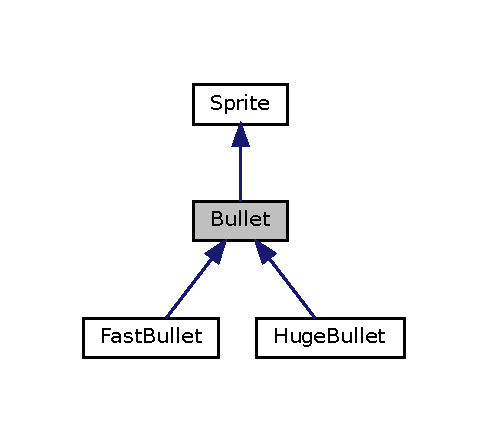
\includegraphics[width=234pt]{classBullet__inherit__graph}
\end{center}
\end{figure}


Collaboration diagram for Bullet\+:
\nopagebreak
\begin{figure}[H]
\begin{center}
\leavevmode
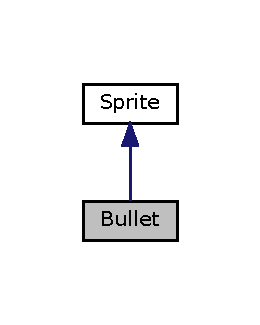
\includegraphics[width=125pt]{classBullet__coll__graph}
\end{center}
\end{figure}
\subsection*{Public Member Functions}
\begin{DoxyCompactItemize}
\item 
\hyperlink{classBullet_ae3b4624da4a6bc8e1fdc595cd5d1514a}{Bullet} (const char $\ast$visual\+\_\+string, const int beg\+\_\+x, const int beg\+\_\+y, const int mom\+\_\+x=0, const int mom\+\_\+y=-\/1)
\item 
virtual \hyperlink{classBullet_aaeb5cb41d7db89f49007b08b41f1bfcf}{$\sim$\+Bullet} ()
\begin{DoxyCompactList}\small\item\em Default destructor. \end{DoxyCompactList}\end{DoxyCompactItemize}
\subsection*{Additional Inherited Members}


\subsection{Detailed Description}
This class serves purpose of being a basic bullet type used for further inheritance. It inherits heavily from class \hyperlink{classSprite}{Sprite} and differs basically only in the default constructor. 

\subsection{Constructor \& Destructor Documentation}
\mbox{\Hypertarget{classBullet_ae3b4624da4a6bc8e1fdc595cd5d1514a}\label{classBullet_ae3b4624da4a6bc8e1fdc595cd5d1514a}} 
\index{Bullet@{Bullet}!Bullet@{Bullet}}
\index{Bullet@{Bullet}!Bullet@{Bullet}}
\subsubsection{\texorpdfstring{Bullet()}{Bullet()}}
{\footnotesize\ttfamily Bullet\+::\+Bullet (\begin{DoxyParamCaption}\item[{const char $\ast$}]{visual\+\_\+string,  }\item[{const int}]{beg\+\_\+x,  }\item[{const int}]{beg\+\_\+y,  }\item[{const int}]{mom\+\_\+x = {\ttfamily 0},  }\item[{const int}]{mom\+\_\+y = {\ttfamily -\/1} }\end{DoxyParamCaption})}

Creates a new instance of a basic bullet


\begin{DoxyParams}{Parameters}
{\em visual\+\_\+string} & String of characters which represents the bullet on the screen. \\
\hline
{\em beg\+\_\+x} & Starting point on X axis for the bullet \\
\hline
{\em beg\+\_\+y} & Starting point on Y axis for the bullet \\
\hline
{\em mom\+\_\+x} & Momentum of the bullet on X axis \\
\hline
{\em mom\+\_\+y} & Momentum of the bullet on Y axis \\
\hline
\end{DoxyParams}
\mbox{\Hypertarget{classBullet_aaeb5cb41d7db89f49007b08b41f1bfcf}\label{classBullet_aaeb5cb41d7db89f49007b08b41f1bfcf}} 
\index{Bullet@{Bullet}!````~Bullet@{$\sim$\+Bullet}}
\index{````~Bullet@{$\sim$\+Bullet}!Bullet@{Bullet}}
\subsubsection{\texorpdfstring{$\sim$\+Bullet()}{~Bullet()}}
{\footnotesize\ttfamily Bullet\+::$\sim$\+Bullet (\begin{DoxyParamCaption}{ }\end{DoxyParamCaption})\hspace{0.3cm}{\ttfamily [virtual]}}



Default destructor. 



The documentation for this class was generated from the following files\+:\begin{DoxyCompactItemize}
\item 
\hyperlink{bullet_8h}{bullet.\+h}\item 
\hyperlink{bullet_8cpp}{bullet.\+cpp}\end{DoxyCompactItemize}

\hypertarget{classCPowerUp}{}\section{C\+Power\+Up Class Reference}
\label{classCPowerUp}\index{C\+Power\+Up@{C\+Power\+Up}}


{\ttfamily \#include $<$power\+\_\+ups.\+h$>$}



Inheritance diagram for C\+Power\+Up\+:
\nopagebreak
\begin{figure}[H]
\begin{center}
\leavevmode
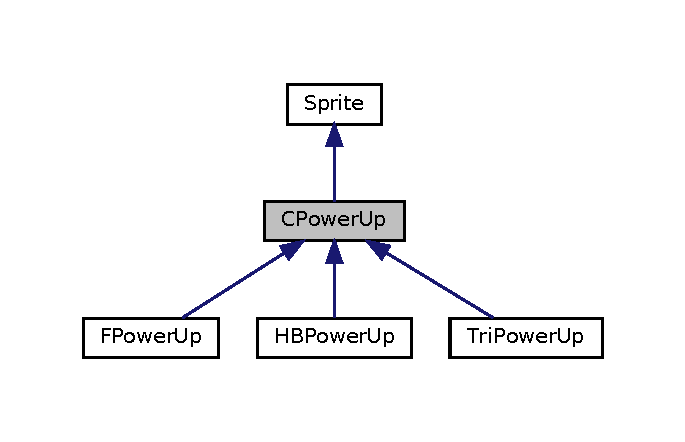
\includegraphics[width=329pt]{classCPowerUp__inherit__graph}
\end{center}
\end{figure}


Collaboration diagram for C\+Power\+Up\+:
\nopagebreak
\begin{figure}[H]
\begin{center}
\leavevmode
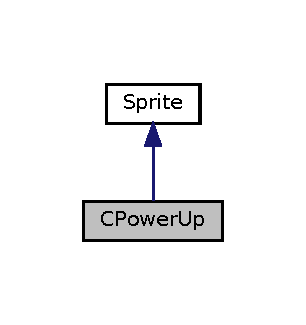
\includegraphics[width=147pt]{classCPowerUp__coll__graph}
\end{center}
\end{figure}
\subsection*{Public Member Functions}
\begin{DoxyCompactItemize}
\item 
\hyperlink{classCPowerUp_ab7f897c487e77f7bbe41af2d0e15ddd4}{C\+Power\+Up} (const int pos\+\_\+x, const int pos\+\_\+y)
\item 
virtual \hyperlink{classCPowerUp_a7c76b245e1c5969add6f8721587817a3}{$\sim$\+C\+Power\+Up} ()
\begin{DoxyCompactList}\small\item\em Default destructor. \end{DoxyCompactList}\item 
int \hyperlink{classCPowerUp_ac934e9e2bebc680caf63c125f75178a8}{get\+Index} () const
\begin{DoxyCompactList}\small\item\em Returns it\textquotesingle{}s own index. \end{DoxyCompactList}\item 
virtual void \hyperlink{classCPowerUp_af1e0bad769efcde21858144596212e01}{draw} (const int timer)
\end{DoxyCompactItemize}
\subsection*{Protected Attributes}
\begin{DoxyCompactItemize}
\item 
int \hyperlink{classCPowerUp_aa8b01cf91f7b24d6d555ae32071bb3bc}{m\+\_\+powerup\+\_\+index}
\begin{DoxyCompactList}\small\item\em Index of the power-\/up. \end{DoxyCompactList}\end{DoxyCompactItemize}


\subsection{Constructor \& Destructor Documentation}
\mbox{\Hypertarget{classCPowerUp_ab7f897c487e77f7bbe41af2d0e15ddd4}\label{classCPowerUp_ab7f897c487e77f7bbe41af2d0e15ddd4}} 
\index{C\+Power\+Up@{C\+Power\+Up}!C\+Power\+Up@{C\+Power\+Up}}
\index{C\+Power\+Up@{C\+Power\+Up}!C\+Power\+Up@{C\+Power\+Up}}
\subsubsection{\texorpdfstring{C\+Power\+Up()}{CPowerUp()}}
{\footnotesize\ttfamily C\+Power\+Up\+::\+C\+Power\+Up (\begin{DoxyParamCaption}\item[{const int}]{pos\+\_\+x,  }\item[{const int}]{pos\+\_\+y }\end{DoxyParamCaption})}

Creates a new instance of a basic power-\/up and sets it\textquotesingle{}s own index.

\begin{DoxyNote}{Note}
It\textquotesingle{}s not really logical, but this power-\/up acts as a \char`\"{}power-\/down\char`\"{}. It\textquotesingle{}s the default shooting method player uses from the beginning. So it\textquotesingle{}s quite slow and shoots only basic bullets.
\end{DoxyNote}

\begin{DoxyParams}{Parameters}
{\em pos\+\_\+x} & Point on the X axis where the power-\/up should be placed \\
\hline
{\em pos\+\_\+y} & Point on the Y axis where the power-\/up should be placed \\
\hline
\end{DoxyParams}
\mbox{\Hypertarget{classCPowerUp_a7c76b245e1c5969add6f8721587817a3}\label{classCPowerUp_a7c76b245e1c5969add6f8721587817a3}} 
\index{C\+Power\+Up@{C\+Power\+Up}!````~C\+Power\+Up@{$\sim$\+C\+Power\+Up}}
\index{````~C\+Power\+Up@{$\sim$\+C\+Power\+Up}!C\+Power\+Up@{C\+Power\+Up}}
\subsubsection{\texorpdfstring{$\sim$\+C\+Power\+Up()}{~CPowerUp()}}
{\footnotesize\ttfamily C\+Power\+Up\+::$\sim$\+C\+Power\+Up (\begin{DoxyParamCaption}{ }\end{DoxyParamCaption})\hspace{0.3cm}{\ttfamily [virtual]}}



Default destructor. 



\subsection{Member Function Documentation}
\mbox{\Hypertarget{classCPowerUp_af1e0bad769efcde21858144596212e01}\label{classCPowerUp_af1e0bad769efcde21858144596212e01}} 
\index{C\+Power\+Up@{C\+Power\+Up}!draw@{draw}}
\index{draw@{draw}!C\+Power\+Up@{C\+Power\+Up}}
\subsubsection{\texorpdfstring{draw()}{draw()}}
{\footnotesize\ttfamily void C\+Power\+Up\+::draw (\begin{DoxyParamCaption}\item[{const int}]{timer }\end{DoxyParamCaption})\hspace{0.3cm}{\ttfamily [virtual]}}

Draws itself on the standard screen. It\textquotesingle{}s overriden because of the different hardcoded color and character it uses as identification.


\begin{DoxyParams}{Parameters}
{\em timer} & Current state of the game\textquotesingle{}s timer. \\
\hline
\end{DoxyParams}


Reimplemented from \hyperlink{classSprite_aa41512617e8a1626bade15cbbdfb3f79}{Sprite}.



Reimplemented in \hyperlink{classFPowerUp_aaf83782b032f53dacd37650127595148}{F\+Power\+Up}, \hyperlink{classHBPowerUp_ac9fcb7d3ef5f3a0561ffe0b6689944a1}{H\+B\+Power\+Up}, and \hyperlink{classTriPowerUp_a06af18b739589c56a90da91716243acf}{Tri\+Power\+Up}.

\mbox{\Hypertarget{classCPowerUp_ac934e9e2bebc680caf63c125f75178a8}\label{classCPowerUp_ac934e9e2bebc680caf63c125f75178a8}} 
\index{C\+Power\+Up@{C\+Power\+Up}!get\+Index@{get\+Index}}
\index{get\+Index@{get\+Index}!C\+Power\+Up@{C\+Power\+Up}}
\subsubsection{\texorpdfstring{get\+Index()}{getIndex()}}
{\footnotesize\ttfamily int C\+Power\+Up\+::get\+Index (\begin{DoxyParamCaption}{ }\end{DoxyParamCaption}) const}



Returns it\textquotesingle{}s own index. 



\subsection{Member Data Documentation}
\mbox{\Hypertarget{classCPowerUp_aa8b01cf91f7b24d6d555ae32071bb3bc}\label{classCPowerUp_aa8b01cf91f7b24d6d555ae32071bb3bc}} 
\index{C\+Power\+Up@{C\+Power\+Up}!m\+\_\+powerup\+\_\+index@{m\+\_\+powerup\+\_\+index}}
\index{m\+\_\+powerup\+\_\+index@{m\+\_\+powerup\+\_\+index}!C\+Power\+Up@{C\+Power\+Up}}
\subsubsection{\texorpdfstring{m\+\_\+powerup\+\_\+index}{m\_powerup\_index}}
{\footnotesize\ttfamily int C\+Power\+Up\+::m\+\_\+powerup\+\_\+index\hspace{0.3cm}{\ttfamily [protected]}}



Index of the power-\/up. 



The documentation for this class was generated from the following files\+:\begin{DoxyCompactItemize}
\item 
\hyperlink{power__ups_8h}{power\+\_\+ups.\+h}\item 
\hyperlink{power__ups_8cpp}{power\+\_\+ups.\+cpp}\end{DoxyCompactItemize}

\hypertarget{classEnemy}{}\section{Enemy Class Reference}
\label{classEnemy}\index{Enemy@{Enemy}}


{\ttfamily \#include $<$enemy.\+h$>$}



Inheritance diagram for Enemy\+:\nopagebreak
\begin{figure}[H]
\begin{center}
\leavevmode
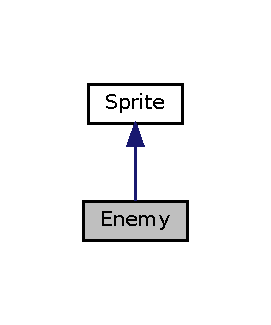
\includegraphics[width=130pt]{classEnemy__inherit__graph}
\end{center}
\end{figure}


Collaboration diagram for Enemy\+:\nopagebreak
\begin{figure}[H]
\begin{center}
\leavevmode
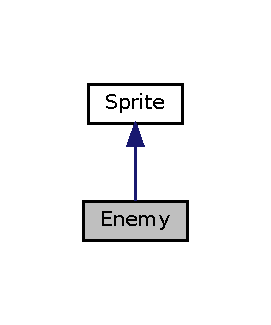
\includegraphics[width=130pt]{classEnemy__coll__graph}
\end{center}
\end{figure}
\subsection*{Public Member Functions}
\begin{DoxyCompactItemize}
\item 
\hyperlink{classEnemy_a4ef7e05685524e2f717879b9428e5534}{Enemy} (const char $\ast$visual\+\_\+string, const int beg\+\_\+x=0, const int beg\+\_\+y=0)
\item 
virtual \hyperlink{classEnemy_ac0eec4755e28c02688065f9657150ac3}{$\sim$\+Enemy} ()
\begin{DoxyCompactList}\small\item\em Default destructor. \end{DoxyCompactList}\end{DoxyCompactItemize}
\subsection*{Additional Inherited Members}


\subsection{Detailed Description}
This class serves purpose of being a basic enemy type. It basically inherits everything from it\textquotesingle{}s parent class -\/ \hyperlink{classSprite}{Sprite}. We only change it\textquotesingle{}s movement direction inside the constructor. 

\subsection{Constructor \& Destructor Documentation}
\mbox{\Hypertarget{classEnemy_a4ef7e05685524e2f717879b9428e5534}\label{classEnemy_a4ef7e05685524e2f717879b9428e5534}} 
\index{Enemy@{Enemy}!Enemy@{Enemy}}
\index{Enemy@{Enemy}!Enemy@{Enemy}}
\subsubsection{\texorpdfstring{Enemy()}{Enemy()}}
{\footnotesize\ttfamily Enemy\+::\+Enemy (\begin{DoxyParamCaption}\item[{const char $\ast$}]{visual\+\_\+string,  }\item[{const int}]{beg\+\_\+x = {\ttfamily 0},  }\item[{const int}]{beg\+\_\+y = {\ttfamily 0} }\end{DoxyParamCaption})}

Creates a new instance of a basic enemy


\begin{DoxyParams}{Parameters}
{\em visual\+\_\+string} & String of characters which represents the enemy on the screen. \\
\hline
{\em beg\+\_\+x} & Starting point on X axis for the enemy \\
\hline
{\em beg\+\_\+y} & Starting point on Y axis for the enemy \\
\hline
\end{DoxyParams}
\mbox{\Hypertarget{classEnemy_ac0eec4755e28c02688065f9657150ac3}\label{classEnemy_ac0eec4755e28c02688065f9657150ac3}} 
\index{Enemy@{Enemy}!````~Enemy@{$\sim$\+Enemy}}
\index{````~Enemy@{$\sim$\+Enemy}!Enemy@{Enemy}}
\subsubsection{\texorpdfstring{$\sim$\+Enemy()}{~Enemy()}}
{\footnotesize\ttfamily Enemy\+::$\sim$\+Enemy (\begin{DoxyParamCaption}{ }\end{DoxyParamCaption})\hspace{0.3cm}{\ttfamily [virtual]}}



Default destructor. 



The documentation for this class was generated from the following files\+:\begin{DoxyCompactItemize}
\item 
\hyperlink{enemy_8h}{enemy.\+h}\item 
\hyperlink{enemy_8cpp}{enemy.\+cpp}\end{DoxyCompactItemize}

\hypertarget{classEngineWrapper}{}\section{Engine\+Wrapper Class Reference}
\label{classEngineWrapper}\index{Engine\+Wrapper@{Engine\+Wrapper}}


{\ttfamily \#include $<$engine.\+h$>$}

\subsection*{Public Member Functions}
\begin{DoxyCompactItemize}
\item 
\hyperlink{classEngineWrapper_a7d136e07dd38ffca1a37de9c35810033}{Engine\+Wrapper} (const int refresh\+\_\+target)
\item 
\hyperlink{classEngineWrapper_afe15effdb74568bc23c189cd8933034d}{$\sim$\+Engine\+Wrapper} ()
\begin{DoxyCompactList}\small\item\em Default destructor. \end{DoxyCompactList}\item 
int \hyperlink{classEngineWrapper_a8f5165549dd3ab6a738d68828c18a3d7}{get\+Screen\+Width} () const
\item 
int \hyperlink{classEngineWrapper_ad308af51b894a88370e5d29933d22e2e}{get\+Screen\+Height} () const
\item 
void \hyperlink{classEngineWrapper_aff72a50573fe66999186d0e258625199}{draw\+All\+Objects} (const int timer, const int score, \hyperlink{classSprite}{Sprite} $\ast$player\+\_\+ref, std\+::list$<$ \hyperlink{classSprite}{Sprite} $\ast$$>$ \&bullets\+\_\+ref, std\+::list$<$ \hyperlink{classSprite}{Sprite} $\ast$$>$ \&enemies\+\_\+ref, std\+::list$<$ \hyperlink{classCPowerUp}{C\+Power\+Up} $\ast$$>$ \&power\+\_\+ups\+\_\+ref)
\begin{DoxyCompactList}\small\item\em Draws all given objects onto the canvas (calls their draw() methods) \end{DoxyCompactList}\item 
void \hyperlink{classEngineWrapper_aa28f572916346dc5b658e83030e412bb}{delete\+Invisible\+Objects} (std\+::list$<$ \hyperlink{classSprite}{Sprite} $\ast$$>$ \&bullets\+\_\+ref, std\+::list$<$ \hyperlink{classSprite}{Sprite} $\ast$$>$ \&enemies\+\_\+ref, std\+::list$<$ \hyperlink{classCPowerUp}{C\+Power\+Up} $\ast$$>$ \&power\+\_\+ups\+\_\+ref)
\item 
void \hyperlink{classEngineWrapper_a3e56de98238ab684cec60aaa556e1e40}{wait\+F\+PS} ()
\begin{DoxyCompactList}\small\item\em Waits for the 1000/targeted\+\_\+framerate milliseconds. \end{DoxyCompactList}\item 
void \hyperlink{classEngineWrapper_ad2e7298e01e58e4ddf4ce34f40b1ef50}{end\+Ncurses} ()
\begin{DoxyCompactList}\small\item\em Tells N\+Curses to end and close the created drawing canvas. \end{DoxyCompactList}\item 
void \hyperlink{classEngineWrapper_a2831a7eb3e2743e72848014314fc7e0e}{load\+Screen\+Dimensions} ()
\begin{DoxyCompactList}\small\item\em Loads screen\textquotesingle{}s dimensions in character blocks (just a wrapper around ncurses call) \end{DoxyCompactList}\end{DoxyCompactItemize}
\subsection*{Private Attributes}
\begin{DoxyCompactItemize}
\item 
int \hyperlink{classEngineWrapper_a53d49d56ab2b6e1ec9d34c2826f09f78}{m\+\_\+screen\+\_\+width}
\begin{DoxyCompactList}\small\item\em Variable to store current screen\textquotesingle{}s width. \end{DoxyCompactList}\item 
int \hyperlink{classEngineWrapper_a493a1f3303ab70c4dc90145e57ea3eaf}{m\+\_\+screen\+\_\+height}
\begin{DoxyCompactList}\small\item\em Variable to store current screen\textquotesingle{}s height. \end{DoxyCompactList}\item 
int \hyperlink{classEngineWrapper_a4a5092ca1f1008be1c49867fc0abd3c8}{m\+\_\+refresh\+\_\+rate}
\begin{DoxyCompactList}\small\item\em How long in milliseconds the engine should wait between each frame (gets calculated automatically) \end{DoxyCompactList}\end{DoxyCompactItemize}


\subsection{Detailed Description}
Mainly a helper class to hide some N\+Curses specific functions and settings 

\subsection{Constructor \& Destructor Documentation}
\mbox{\Hypertarget{classEngineWrapper_a7d136e07dd38ffca1a37de9c35810033}\label{classEngineWrapper_a7d136e07dd38ffca1a37de9c35810033}} 
\index{Engine\+Wrapper@{Engine\+Wrapper}!Engine\+Wrapper@{Engine\+Wrapper}}
\index{Engine\+Wrapper@{Engine\+Wrapper}!Engine\+Wrapper@{Engine\+Wrapper}}
\subsubsection{\texorpdfstring{Engine\+Wrapper()}{EngineWrapper()}}
{\footnotesize\ttfamily Engine\+Wrapper\+::\+Engine\+Wrapper (\begin{DoxyParamCaption}\item[{const int}]{refresh\+\_\+target }\end{DoxyParamCaption})}

Creates a new instance of out engine


\begin{DoxyParams}{Parameters}
{\em refresh\+\_\+target} & Target amount of frames per second the engine should try to accomplish \\
\hline
\end{DoxyParams}
\mbox{\Hypertarget{classEngineWrapper_afe15effdb74568bc23c189cd8933034d}\label{classEngineWrapper_afe15effdb74568bc23c189cd8933034d}} 
\index{Engine\+Wrapper@{Engine\+Wrapper}!````~Engine\+Wrapper@{$\sim$\+Engine\+Wrapper}}
\index{````~Engine\+Wrapper@{$\sim$\+Engine\+Wrapper}!Engine\+Wrapper@{Engine\+Wrapper}}
\subsubsection{\texorpdfstring{$\sim$\+Engine\+Wrapper()}{~EngineWrapper()}}
{\footnotesize\ttfamily Engine\+Wrapper\+::$\sim$\+Engine\+Wrapper (\begin{DoxyParamCaption}{ }\end{DoxyParamCaption})}



Default destructor. 



\subsection{Member Function Documentation}
\mbox{\Hypertarget{classEngineWrapper_aa28f572916346dc5b658e83030e412bb}\label{classEngineWrapper_aa28f572916346dc5b658e83030e412bb}} 
\index{Engine\+Wrapper@{Engine\+Wrapper}!delete\+Invisible\+Objects@{delete\+Invisible\+Objects}}
\index{delete\+Invisible\+Objects@{delete\+Invisible\+Objects}!Engine\+Wrapper@{Engine\+Wrapper}}
\subsubsection{\texorpdfstring{delete\+Invisible\+Objects()}{deleteInvisibleObjects()}}
{\footnotesize\ttfamily void Engine\+Wrapper\+::delete\+Invisible\+Objects (\begin{DoxyParamCaption}\item[{std\+::list$<$ \hyperlink{classSprite}{Sprite} $\ast$$>$ \&}]{bullets\+\_\+ref,  }\item[{std\+::list$<$ \hyperlink{classSprite}{Sprite} $\ast$$>$ \&}]{enemies\+\_\+ref,  }\item[{std\+::list$<$ \hyperlink{classCPowerUp}{C\+Power\+Up} $\ast$$>$ \&}]{power\+\_\+ups\+\_\+ref }\end{DoxyParamCaption})}

Goes though each given list, removes and deletes any invisible object it finds


\begin{DoxyParams}{Parameters}
{\em bullets\+\_\+ref} & Reference to the list of (in)visible bullets \\
\hline
{\em enemies\+\_\+ref} & Reference to the list of (in)visible enemies \\
\hline
{\em power\+\_\+ups\+\_\+ref} & Reference to the list of (in)visible power-\/ups \\
\hline
\end{DoxyParams}
\mbox{\Hypertarget{classEngineWrapper_aff72a50573fe66999186d0e258625199}\label{classEngineWrapper_aff72a50573fe66999186d0e258625199}} 
\index{Engine\+Wrapper@{Engine\+Wrapper}!draw\+All\+Objects@{draw\+All\+Objects}}
\index{draw\+All\+Objects@{draw\+All\+Objects}!Engine\+Wrapper@{Engine\+Wrapper}}
\subsubsection{\texorpdfstring{draw\+All\+Objects()}{drawAllObjects()}}
{\footnotesize\ttfamily void Engine\+Wrapper\+::draw\+All\+Objects (\begin{DoxyParamCaption}\item[{const int}]{timer,  }\item[{const int}]{score,  }\item[{\hyperlink{classSprite}{Sprite} $\ast$}]{player\+\_\+ref,  }\item[{std\+::list$<$ \hyperlink{classSprite}{Sprite} $\ast$$>$ \&}]{bullets\+\_\+ref,  }\item[{std\+::list$<$ \hyperlink{classSprite}{Sprite} $\ast$$>$ \&}]{enemies\+\_\+ref,  }\item[{std\+::list$<$ \hyperlink{classCPowerUp}{C\+Power\+Up} $\ast$$>$ \&}]{power\+\_\+ups\+\_\+ref }\end{DoxyParamCaption})}



Draws all given objects onto the canvas (calls their draw() methods) 

\begin{DoxyNote}{Note}
Yes, it\textquotesingle{}s a bit cumbersome to have so many of our case specific arguments.
\end{DoxyNote}
Goes through all the given lists and calls draw() on each of its members. Plus it draws current score of the player. Handy to remind that the draw() method also recalculates the objects new location.


\begin{DoxyParams}{Parameters}
{\em timer} & Current state of the game\textquotesingle{}s timer \\
\hline
{\em score} & Current player\textquotesingle{}s score \\
\hline
{\em player\+\_\+ref} & Pointer to the player object \\
\hline
{\em bullets\+\_\+ref} & Reference to the list of visible bullets \\
\hline
{\em enemies\+\_\+ref} & Reference to the list of visible enemies \\
\hline
{\em power\+\_\+ups\+\_\+ref} & Reference to the list of visible power-\/ups \\
\hline
\end{DoxyParams}
\mbox{\Hypertarget{classEngineWrapper_ad2e7298e01e58e4ddf4ce34f40b1ef50}\label{classEngineWrapper_ad2e7298e01e58e4ddf4ce34f40b1ef50}} 
\index{Engine\+Wrapper@{Engine\+Wrapper}!end\+Ncurses@{end\+Ncurses}}
\index{end\+Ncurses@{end\+Ncurses}!Engine\+Wrapper@{Engine\+Wrapper}}
\subsubsection{\texorpdfstring{end\+Ncurses()}{endNcurses()}}
{\footnotesize\ttfamily void Engine\+Wrapper\+::end\+Ncurses (\begin{DoxyParamCaption}{ }\end{DoxyParamCaption})}



Tells N\+Curses to end and close the created drawing canvas. 

\mbox{\Hypertarget{classEngineWrapper_ad308af51b894a88370e5d29933d22e2e}\label{classEngineWrapper_ad308af51b894a88370e5d29933d22e2e}} 
\index{Engine\+Wrapper@{Engine\+Wrapper}!get\+Screen\+Height@{get\+Screen\+Height}}
\index{get\+Screen\+Height@{get\+Screen\+Height}!Engine\+Wrapper@{Engine\+Wrapper}}
\subsubsection{\texorpdfstring{get\+Screen\+Height()}{getScreenHeight()}}
{\footnotesize\ttfamily int Engine\+Wrapper\+::get\+Screen\+Height (\begin{DoxyParamCaption}{ }\end{DoxyParamCaption}) const}

Returns currently stored screen\textquotesingle{}s height

\begin{DoxyReturn}{Returns}
Lastly gotten screen\textquotesingle{}s height in character blocks 
\end{DoxyReturn}
\mbox{\Hypertarget{classEngineWrapper_a8f5165549dd3ab6a738d68828c18a3d7}\label{classEngineWrapper_a8f5165549dd3ab6a738d68828c18a3d7}} 
\index{Engine\+Wrapper@{Engine\+Wrapper}!get\+Screen\+Width@{get\+Screen\+Width}}
\index{get\+Screen\+Width@{get\+Screen\+Width}!Engine\+Wrapper@{Engine\+Wrapper}}
\subsubsection{\texorpdfstring{get\+Screen\+Width()}{getScreenWidth()}}
{\footnotesize\ttfamily int Engine\+Wrapper\+::get\+Screen\+Width (\begin{DoxyParamCaption}{ }\end{DoxyParamCaption}) const}

Returns currently stored screen\textquotesingle{}s width

\begin{DoxyReturn}{Returns}
Lastly gotten screen\textquotesingle{}s width in character blocks 
\end{DoxyReturn}
\mbox{\Hypertarget{classEngineWrapper_a2831a7eb3e2743e72848014314fc7e0e}\label{classEngineWrapper_a2831a7eb3e2743e72848014314fc7e0e}} 
\index{Engine\+Wrapper@{Engine\+Wrapper}!load\+Screen\+Dimensions@{load\+Screen\+Dimensions}}
\index{load\+Screen\+Dimensions@{load\+Screen\+Dimensions}!Engine\+Wrapper@{Engine\+Wrapper}}
\subsubsection{\texorpdfstring{load\+Screen\+Dimensions()}{loadScreenDimensions()}}
{\footnotesize\ttfamily void Engine\+Wrapper\+::load\+Screen\+Dimensions (\begin{DoxyParamCaption}{ }\end{DoxyParamCaption})}



Loads screen\textquotesingle{}s dimensions in character blocks (just a wrapper around ncurses call) 

\mbox{\Hypertarget{classEngineWrapper_a3e56de98238ab684cec60aaa556e1e40}\label{classEngineWrapper_a3e56de98238ab684cec60aaa556e1e40}} 
\index{Engine\+Wrapper@{Engine\+Wrapper}!wait\+F\+PS@{wait\+F\+PS}}
\index{wait\+F\+PS@{wait\+F\+PS}!Engine\+Wrapper@{Engine\+Wrapper}}
\subsubsection{\texorpdfstring{wait\+F\+P\+S()}{waitFPS()}}
{\footnotesize\ttfamily void Engine\+Wrapper\+::wait\+F\+PS (\begin{DoxyParamCaption}{ }\end{DoxyParamCaption})}



Waits for the 1000/targeted\+\_\+framerate milliseconds. 



\subsection{Member Data Documentation}
\mbox{\Hypertarget{classEngineWrapper_a4a5092ca1f1008be1c49867fc0abd3c8}\label{classEngineWrapper_a4a5092ca1f1008be1c49867fc0abd3c8}} 
\index{Engine\+Wrapper@{Engine\+Wrapper}!m\+\_\+refresh\+\_\+rate@{m\+\_\+refresh\+\_\+rate}}
\index{m\+\_\+refresh\+\_\+rate@{m\+\_\+refresh\+\_\+rate}!Engine\+Wrapper@{Engine\+Wrapper}}
\subsubsection{\texorpdfstring{m\+\_\+refresh\+\_\+rate}{m\_refresh\_rate}}
{\footnotesize\ttfamily int Engine\+Wrapper\+::m\+\_\+refresh\+\_\+rate\hspace{0.3cm}{\ttfamily [private]}}



How long in milliseconds the engine should wait between each frame (gets calculated automatically) 

\mbox{\Hypertarget{classEngineWrapper_a493a1f3303ab70c4dc90145e57ea3eaf}\label{classEngineWrapper_a493a1f3303ab70c4dc90145e57ea3eaf}} 
\index{Engine\+Wrapper@{Engine\+Wrapper}!m\+\_\+screen\+\_\+height@{m\+\_\+screen\+\_\+height}}
\index{m\+\_\+screen\+\_\+height@{m\+\_\+screen\+\_\+height}!Engine\+Wrapper@{Engine\+Wrapper}}
\subsubsection{\texorpdfstring{m\+\_\+screen\+\_\+height}{m\_screen\_height}}
{\footnotesize\ttfamily int Engine\+Wrapper\+::m\+\_\+screen\+\_\+height\hspace{0.3cm}{\ttfamily [private]}}



Variable to store current screen\textquotesingle{}s height. 

\mbox{\Hypertarget{classEngineWrapper_a53d49d56ab2b6e1ec9d34c2826f09f78}\label{classEngineWrapper_a53d49d56ab2b6e1ec9d34c2826f09f78}} 
\index{Engine\+Wrapper@{Engine\+Wrapper}!m\+\_\+screen\+\_\+width@{m\+\_\+screen\+\_\+width}}
\index{m\+\_\+screen\+\_\+width@{m\+\_\+screen\+\_\+width}!Engine\+Wrapper@{Engine\+Wrapper}}
\subsubsection{\texorpdfstring{m\+\_\+screen\+\_\+width}{m\_screen\_width}}
{\footnotesize\ttfamily int Engine\+Wrapper\+::m\+\_\+screen\+\_\+width\hspace{0.3cm}{\ttfamily [private]}}



Variable to store current screen\textquotesingle{}s width. 



The documentation for this class was generated from the following files\+:\begin{DoxyCompactItemize}
\item 
\hyperlink{engine_8h}{engine.\+h}\item 
\hyperlink{engine_8cpp}{engine.\+cpp}\end{DoxyCompactItemize}

\hypertarget{classFastBullet}{}\section{Fast\+Bullet Class Reference}
\label{classFastBullet}\index{Fast\+Bullet@{Fast\+Bullet}}


{\ttfamily \#include $<$bullet\+\_\+fast.\+h$>$}



Inheritance diagram for Fast\+Bullet\+:
\nopagebreak
\begin{figure}[H]
\begin{center}
\leavevmode
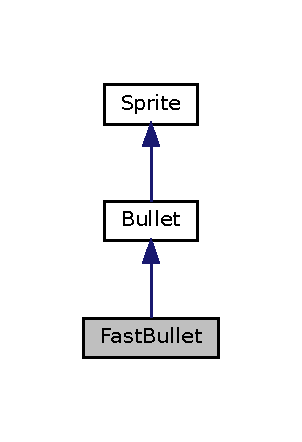
\includegraphics[width=145pt]{classFastBullet__inherit__graph}
\end{center}
\end{figure}


Collaboration diagram for Fast\+Bullet\+:
\nopagebreak
\begin{figure}[H]
\begin{center}
\leavevmode
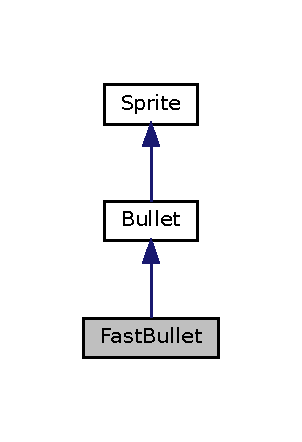
\includegraphics[width=145pt]{classFastBullet__coll__graph}
\end{center}
\end{figure}
\subsection*{Public Member Functions}
\begin{DoxyCompactItemize}
\item 
\hyperlink{classFastBullet_ae8800f319fabc46ec8c44f23aa21c485}{Fast\+Bullet} (const int beg\+\_\+x, const int beg\+\_\+y, const int mom\+\_\+x=0, const int mom\+\_\+y=-\/1)
\item 
\hyperlink{classFastBullet_a276249fe2605b4b3706eee2e33e2b152}{$\sim$\+Fast\+Bullet} ()
\begin{DoxyCompactList}\small\item\em Default destructor. \end{DoxyCompactList}\end{DoxyCompactItemize}
\subsection*{Additional Inherited Members}


\subsection{Detailed Description}
This class serves purpose of being the default bullet for \hyperlink{classFPowerUp}{F\+Power\+Up}. Compared to basic \hyperlink{classBullet}{Bullet}, it has an increase speed of movement, accomplished by being redrawn every tick of the game\textquotesingle{}s timer. It inherits heavily from it\textquotesingle{}s parent class -\/ \hyperlink{classBullet}{Bullet} and differs only in the default constructor. 

\subsection{Constructor \& Destructor Documentation}
\mbox{\Hypertarget{classFastBullet_ae8800f319fabc46ec8c44f23aa21c485}\label{classFastBullet_ae8800f319fabc46ec8c44f23aa21c485}} 
\index{Fast\+Bullet@{Fast\+Bullet}!Fast\+Bullet@{Fast\+Bullet}}
\index{Fast\+Bullet@{Fast\+Bullet}!Fast\+Bullet@{Fast\+Bullet}}
\subsubsection{\texorpdfstring{Fast\+Bullet()}{FastBullet()}}
{\footnotesize\ttfamily Fast\+Bullet\+::\+Fast\+Bullet (\begin{DoxyParamCaption}\item[{const int}]{beg\+\_\+x,  }\item[{const int}]{beg\+\_\+y,  }\item[{const int}]{mom\+\_\+x = {\ttfamily 0},  }\item[{const int}]{mom\+\_\+y = {\ttfamily -\/1} }\end{DoxyParamCaption})}

Creates a new instance of a fast travelling bullet \begin{DoxyNote}{Note}
Compared to \hyperlink{classBullet}{Bullet}, it doesn\textquotesingle{}t use a visual\+\_\+string parameter as it is hardcoded into the class.
\end{DoxyNote}

\begin{DoxyParams}{Parameters}
{\em beg\+\_\+x} & Starting point on X axis for the bullet \\
\hline
{\em beg\+\_\+y} & Starting point on Y axis for the bullet \\
\hline
{\em mom\+\_\+x} & Momentum of the bullet on X axis \\
\hline
{\em mom\+\_\+y} & Momentum of the bullet on Y axis \\
\hline
\end{DoxyParams}
\mbox{\Hypertarget{classFastBullet_a276249fe2605b4b3706eee2e33e2b152}\label{classFastBullet_a276249fe2605b4b3706eee2e33e2b152}} 
\index{Fast\+Bullet@{Fast\+Bullet}!````~Fast\+Bullet@{$\sim$\+Fast\+Bullet}}
\index{````~Fast\+Bullet@{$\sim$\+Fast\+Bullet}!Fast\+Bullet@{Fast\+Bullet}}
\subsubsection{\texorpdfstring{$\sim$\+Fast\+Bullet()}{~FastBullet()}}
{\footnotesize\ttfamily Fast\+Bullet\+::$\sim$\+Fast\+Bullet (\begin{DoxyParamCaption}{ }\end{DoxyParamCaption})}



Default destructor. 



The documentation for this class was generated from the following files\+:\begin{DoxyCompactItemize}
\item 
\hyperlink{bullet__fast_8h}{bullet\+\_\+fast.\+h}\item 
\hyperlink{bullet__fast_8cpp}{bullet\+\_\+fast.\+cpp}\end{DoxyCompactItemize}

\hypertarget{classFPowerUp}{}\section{F\+Power\+Up Class Reference}
\label{classFPowerUp}\index{F\+Power\+Up@{F\+Power\+Up}}


{\ttfamily \#include $<$power\+\_\+ups.\+h$>$}



Inheritance diagram for F\+Power\+Up\+:
\nopagebreak
\begin{figure}[H]
\begin{center}
\leavevmode
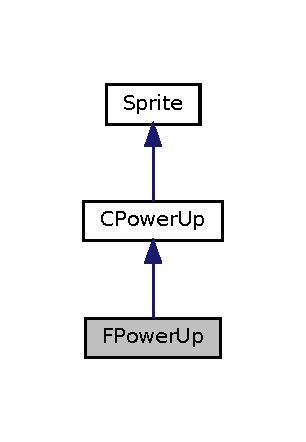
\includegraphics[width=147pt]{classFPowerUp__inherit__graph}
\end{center}
\end{figure}


Collaboration diagram for F\+Power\+Up\+:
\nopagebreak
\begin{figure}[H]
\begin{center}
\leavevmode
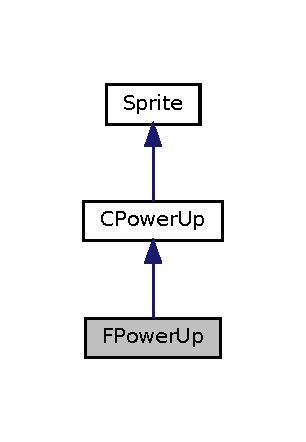
\includegraphics[width=147pt]{classFPowerUp__coll__graph}
\end{center}
\end{figure}
\subsection*{Public Member Functions}
\begin{DoxyCompactItemize}
\item 
\hyperlink{classFPowerUp_a7377a01b8c39b7342fdb457e6635833c}{F\+Power\+Up} (const int pos\+\_\+x, const int pos\+\_\+y)
\item 
\hyperlink{classFPowerUp_aa062fd6a8f23d57dcb4e282583f3bfc8}{$\sim$\+F\+Power\+Up} ()
\begin{DoxyCompactList}\small\item\em Default destructor. \end{DoxyCompactList}\item 
void \hyperlink{classFPowerUp_aaf83782b032f53dacd37650127595148}{draw} (const int timer)
\end{DoxyCompactItemize}
\subsection*{Additional Inherited Members}


\subsection{Detailed Description}
This header file hosts all of the power-\/ups at the same time. I did it because of how small the differences between the power-\/ups are.

\hyperlink{classCPowerUp}{C\+Power\+Up} acts as the parent\textquotesingle{}s class. It inherits directly from \hyperlink{classSprite}{Sprite}. 

\subsection{Constructor \& Destructor Documentation}
\mbox{\Hypertarget{classFPowerUp_a7377a01b8c39b7342fdb457e6635833c}\label{classFPowerUp_a7377a01b8c39b7342fdb457e6635833c}} 
\index{F\+Power\+Up@{F\+Power\+Up}!F\+Power\+Up@{F\+Power\+Up}}
\index{F\+Power\+Up@{F\+Power\+Up}!F\+Power\+Up@{F\+Power\+Up}}
\subsubsection{\texorpdfstring{F\+Power\+Up()}{FPowerUp()}}
{\footnotesize\ttfamily F\+Power\+Up\+::\+F\+Power\+Up (\begin{DoxyParamCaption}\item[{const int}]{pos\+\_\+x,  }\item[{const int}]{pos\+\_\+y }\end{DoxyParamCaption})}

Creates a new instance of a Fast-\/\+Bullet power-\/up and sets it\textquotesingle{}s own index.


\begin{DoxyParams}{Parameters}
{\em pos\+\_\+x} & Point on the X axis where the power-\/up should be placed \\
\hline
{\em pos\+\_\+y} & Point on the Y axis where the power-\/up should be placed \\
\hline
\end{DoxyParams}
\mbox{\Hypertarget{classFPowerUp_aa062fd6a8f23d57dcb4e282583f3bfc8}\label{classFPowerUp_aa062fd6a8f23d57dcb4e282583f3bfc8}} 
\index{F\+Power\+Up@{F\+Power\+Up}!````~F\+Power\+Up@{$\sim$\+F\+Power\+Up}}
\index{````~F\+Power\+Up@{$\sim$\+F\+Power\+Up}!F\+Power\+Up@{F\+Power\+Up}}
\subsubsection{\texorpdfstring{$\sim$\+F\+Power\+Up()}{~FPowerUp()}}
{\footnotesize\ttfamily F\+Power\+Up\+::$\sim$\+F\+Power\+Up (\begin{DoxyParamCaption}{ }\end{DoxyParamCaption})}



Default destructor. 



\subsection{Member Function Documentation}
\mbox{\Hypertarget{classFPowerUp_aaf83782b032f53dacd37650127595148}\label{classFPowerUp_aaf83782b032f53dacd37650127595148}} 
\index{F\+Power\+Up@{F\+Power\+Up}!draw@{draw}}
\index{draw@{draw}!F\+Power\+Up@{F\+Power\+Up}}
\subsubsection{\texorpdfstring{draw()}{draw()}}
{\footnotesize\ttfamily void F\+Power\+Up\+::draw (\begin{DoxyParamCaption}\item[{const int}]{timer }\end{DoxyParamCaption})\hspace{0.3cm}{\ttfamily [virtual]}}

Draws itself on the standard screen. It\textquotesingle{}s overriden because of the different hardcoded color and character it uses as identification.


\begin{DoxyParams}{Parameters}
{\em timer} & Current state of the game\textquotesingle{}s timer. \\
\hline
\end{DoxyParams}


Reimplemented from \hyperlink{classCPowerUp_af1e0bad769efcde21858144596212e01}{C\+Power\+Up}.



The documentation for this class was generated from the following files\+:\begin{DoxyCompactItemize}
\item 
\hyperlink{power__ups_8h}{power\+\_\+ups.\+h}\item 
\hyperlink{power__ups_8cpp}{power\+\_\+ups.\+cpp}\end{DoxyCompactItemize}

\hypertarget{classGeus}{}\section{Geus Class Reference}
\label{classGeus}\index{Geus@{Geus}}


{\ttfamily \#include $<$geus.\+h$>$}



Collaboration diagram for Geus\+:
\nopagebreak
\begin{figure}[H]
\begin{center}
\leavevmode
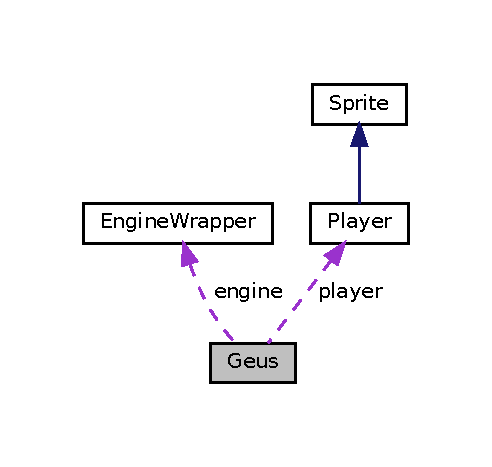
\includegraphics[width=236pt]{classGeus__coll__graph}
\end{center}
\end{figure}
\subsection*{Public Member Functions}
\begin{DoxyCompactItemize}
\item 
\hyperlink{classGeus_a21852cfcb9229ce95773f15cf1e8620e}{Geus} ()
\begin{DoxyCompactList}\small\item\em Default constructor. \end{DoxyCompactList}\item 
\hyperlink{classGeus_ac6a5d703343da401f4af4c9eb89a5ae8}{$\sim$\+Geus} ()
\begin{DoxyCompactList}\small\item\em Default destructor. \end{DoxyCompactList}\item 
int \hyperlink{classGeus_af62245e002ed29f52e4ffff6372f4da9}{play} ()
\end{DoxyCompactItemize}
\subsection*{Private Member Functions}
\begin{DoxyCompactItemize}
\item 
void \hyperlink{classGeus_ac562cba645d11b3ead596a40f2138ae8}{handle\+Input} ()
\begin{DoxyCompactList}\small\item\em Function used to check the currently pressed key and link it to a corresponding action. \end{DoxyCompactList}\item 
void \hyperlink{classGeus_a203be0301bb8cf927691e104184a9d1a}{load\+Enemy\+Positions} (const char $\ast$file\+\_\+path)
\item 
void \hyperlink{classGeus_a2992ad2cc9b243e28a0f344721ac217d}{load\+Line\+Of\+Enemies} ()
\item 
void \hyperlink{classGeus_a9543c5d421c0a5926bfb16d59bbcab12}{random\+Drop\+Power\+Up} (const int pos\+\_\+x, const int pos\+\_\+y)
\begin{DoxyCompactList}\small\item\em Drops a random power-\/up based on hardcoded probability. \end{DoxyCompactList}\item 
void \hyperlink{classGeus_a43863016c0866aae15e64994c6f4f45f}{load\+Highest\+Score} ()
\begin{DoxyCompactList}\small\item\em Loads the highest achieved score from a hardcoded file. \end{DoxyCompactList}\item 
void \hyperlink{classGeus_ac39cd26c767b6508030a3a203de80ade}{save\+Highest\+Score} ()
\begin{DoxyCompactList}\small\item\em Saves the current score as the new Highest Score to a hardcoded file. \end{DoxyCompactList}\item 
void \hyperlink{classGeus_a53d54fe777e1eeecbfcd64c852b5322a}{check\+Damage} ()
\begin{DoxyCompactList}\small\item\em Iterates through all of our objects and maps their overlaps between each other to corresponding actions. \end{DoxyCompactList}\item 
void \hyperlink{classGeus_a1325fd4454fd45be398e140b3bcc1120}{end\+Of\+The\+Game\+Screen} (const char $\ast$message)
\end{DoxyCompactItemize}
\subsection*{Private Attributes}
\begin{DoxyCompactItemize}
\item 
\hyperlink{classEngineWrapper}{Engine\+Wrapper} \hyperlink{classGeus_a8b87135ab61453d81b02b97d73033c92}{engine}
\begin{DoxyCompactList}\small\item\em Instance of the engine. \end{DoxyCompactList}\item 
\hyperlink{classPlayer}{Player} $\ast$ \hyperlink{classGeus_a19106a3619fcb55de45bc8adac57496a}{player} = N\+U\+LL
\begin{DoxyCompactList}\small\item\em Single instance of the player\textquotesingle{}s object. \end{DoxyCompactList}\item 
std\+::list$<$ \hyperlink{classSprite}{Sprite} $\ast$ $>$ \hyperlink{classGeus_a182b15c0dcf2def10eb8f084b4e6ce4f}{enemies}
\begin{DoxyCompactList}\small\item\em List with pointers to all visible enemies. \end{DoxyCompactList}\item 
std\+::list$<$ \hyperlink{classSprite}{Sprite} $\ast$ $>$ \hyperlink{classGeus_a48aec553db9de3be3f1cbf0a8d14a1c8}{bullets}
\begin{DoxyCompactList}\small\item\em List with pointers to all visible bullets. \end{DoxyCompactList}\item 
std\+::list$<$ \hyperlink{classCPowerUp}{C\+Power\+Up} $\ast$ $>$ \hyperlink{classGeus_a797d5c7822b9b1e1eb6c46fca93551a3}{power\+\_\+ups}
\item 
std\+::list$<$ int $>$ \hyperlink{classGeus_a2ecbe7a824604651a704e0fff0a5c839}{enemy\+\_\+positions}
\item 
int \hyperlink{classGeus_a8b9366af73b19d4c2383b42e8c5cae7f}{highest\+\_\+score}
\begin{DoxyCompactList}\small\item\em Highest score loaded from a file. \end{DoxyCompactList}\item 
int \hyperlink{classGeus_a2ad271a665a5442697299b756cfee290}{score}
\begin{DoxyCompactList}\small\item\em Current score. \end{DoxyCompactList}\item 
bool \hyperlink{classGeus_aeb4cc6648c47d83e07340b39c85b62b3}{is\+\_\+running}
\begin{DoxyCompactList}\small\item\em A boolean variable controlling the main game loop. \end{DoxyCompactList}\end{DoxyCompactItemize}


\subsection{Detailed Description}
This class serves as the main game class. Here is where all the magic happens. Some of the work is offloaded to the Engine.\+h. That\textquotesingle{}s done solely to make the corresponding .cpp file for this class smaller and a bit easier to read. 

\subsection{Constructor \& Destructor Documentation}
\mbox{\Hypertarget{classGeus_a21852cfcb9229ce95773f15cf1e8620e}\label{classGeus_a21852cfcb9229ce95773f15cf1e8620e}} 
\index{Geus@{Geus}!Geus@{Geus}}
\index{Geus@{Geus}!Geus@{Geus}}
\subsubsection{\texorpdfstring{Geus()}{Geus()}}
{\footnotesize\ttfamily Geus\+::\+Geus (\begin{DoxyParamCaption}{ }\end{DoxyParamCaption})}



Default constructor. 

On creation, creates an instance of \hyperlink{classEngineWrapper}{Engine\+Wrapper} (engine), calculates terminal size, creates an instance of \hyperlink{classPlayer}{Player}, resets current score. \mbox{\Hypertarget{classGeus_ac6a5d703343da401f4af4c9eb89a5ae8}\label{classGeus_ac6a5d703343da401f4af4c9eb89a5ae8}} 
\index{Geus@{Geus}!````~Geus@{$\sim$\+Geus}}
\index{````~Geus@{$\sim$\+Geus}!Geus@{Geus}}
\subsubsection{\texorpdfstring{$\sim$\+Geus()}{~Geus()}}
{\footnotesize\ttfamily Geus\+::$\sim$\+Geus (\begin{DoxyParamCaption}{ }\end{DoxyParamCaption})}



Default destructor. 

Deletes and cleans out three lists of pointers + player 

\subsection{Member Function Documentation}
\mbox{\Hypertarget{classGeus_a53d54fe777e1eeecbfcd64c852b5322a}\label{classGeus_a53d54fe777e1eeecbfcd64c852b5322a}} 
\index{Geus@{Geus}!check\+Damage@{check\+Damage}}
\index{check\+Damage@{check\+Damage}!Geus@{Geus}}
\subsubsection{\texorpdfstring{check\+Damage()}{checkDamage()}}
{\footnotesize\ttfamily void Geus\+::check\+Damage (\begin{DoxyParamCaption}{ }\end{DoxyParamCaption})\hspace{0.3cm}{\ttfamily [private]}}



Iterates through all of our objects and maps their overlaps between each other to corresponding actions. 

\mbox{\Hypertarget{classGeus_a1325fd4454fd45be398e140b3bcc1120}\label{classGeus_a1325fd4454fd45be398e140b3bcc1120}} 
\index{Geus@{Geus}!end\+Of\+The\+Game\+Screen@{end\+Of\+The\+Game\+Screen}}
\index{end\+Of\+The\+Game\+Screen@{end\+Of\+The\+Game\+Screen}!Geus@{Geus}}
\subsubsection{\texorpdfstring{end\+Of\+The\+Game\+Screen()}{endOfTheGameScreen()}}
{\footnotesize\ttfamily void Geus\+::end\+Of\+The\+Game\+Screen (\begin{DoxyParamCaption}\item[{const char $\ast$}]{message }\end{DoxyParamCaption})\hspace{0.3cm}{\ttfamily [private]}}

Displays a message with current score and highest score.

It\textquotesingle{}s being used the last message of the game and can be opened with either a death of the player or press of the E\+SC key

It automatically saves the current score if it\textquotesingle{}s higher than the highest score.


\begin{DoxyParams}{Parameters}
{\em message} & Message to be displayed \\
\hline
\end{DoxyParams}
\mbox{\Hypertarget{classGeus_ac562cba645d11b3ead596a40f2138ae8}\label{classGeus_ac562cba645d11b3ead596a40f2138ae8}} 
\index{Geus@{Geus}!handle\+Input@{handle\+Input}}
\index{handle\+Input@{handle\+Input}!Geus@{Geus}}
\subsubsection{\texorpdfstring{handle\+Input()}{handleInput()}}
{\footnotesize\ttfamily void Geus\+::handle\+Input (\begin{DoxyParamCaption}{ }\end{DoxyParamCaption})\hspace{0.3cm}{\ttfamily [private]}}



Function used to check the currently pressed key and link it to a corresponding action. 

\mbox{\Hypertarget{classGeus_a203be0301bb8cf927691e104184a9d1a}\label{classGeus_a203be0301bb8cf927691e104184a9d1a}} 
\index{Geus@{Geus}!load\+Enemy\+Positions@{load\+Enemy\+Positions}}
\index{load\+Enemy\+Positions@{load\+Enemy\+Positions}!Geus@{Geus}}
\subsubsection{\texorpdfstring{load\+Enemy\+Positions()}{loadEnemyPositions()}}
{\footnotesize\ttfamily void Geus\+::load\+Enemy\+Positions (\begin{DoxyParamCaption}\item[{const char $\ast$}]{file\+\_\+path }\end{DoxyParamCaption})\hspace{0.3cm}{\ttfamily [private]}}

Function which loads enemy positions from a given file and saves it to our list with enemy positions. \begin{DoxyNote}{Note}
In the current state, the file has to exist and be accessible to the program, otherwise an exception is thrown.
\end{DoxyNote}

\begin{DoxyParams}{Parameters}
{\em file\+\_\+path} & Path to a file with enemy positions \\
\hline
\end{DoxyParams}
\mbox{\Hypertarget{classGeus_a43863016c0866aae15e64994c6f4f45f}\label{classGeus_a43863016c0866aae15e64994c6f4f45f}} 
\index{Geus@{Geus}!load\+Highest\+Score@{load\+Highest\+Score}}
\index{load\+Highest\+Score@{load\+Highest\+Score}!Geus@{Geus}}
\subsubsection{\texorpdfstring{load\+Highest\+Score()}{loadHighestScore()}}
{\footnotesize\ttfamily void Geus\+::load\+Highest\+Score (\begin{DoxyParamCaption}{ }\end{DoxyParamCaption})\hspace{0.3cm}{\ttfamily [private]}}



Loads the highest achieved score from a hardcoded file. 

\mbox{\Hypertarget{classGeus_a2992ad2cc9b243e28a0f344721ac217d}\label{classGeus_a2992ad2cc9b243e28a0f344721ac217d}} 
\index{Geus@{Geus}!load\+Line\+Of\+Enemies@{load\+Line\+Of\+Enemies}}
\index{load\+Line\+Of\+Enemies@{load\+Line\+Of\+Enemies}!Geus@{Geus}}
\subsubsection{\texorpdfstring{load\+Line\+Of\+Enemies()}{loadLineOfEnemies()}}
{\footnotesize\ttfamily void Geus\+::load\+Line\+Of\+Enemies (\begin{DoxyParamCaption}{ }\end{DoxyParamCaption})\hspace{0.3cm}{\ttfamily [private]}}

Loads one line of enemies from our list with enemy positions, creates new enemies, saves them to the corresponding \char`\"{}enemies\char`\"{} list. \mbox{\Hypertarget{classGeus_af62245e002ed29f52e4ffff6372f4da9}\label{classGeus_af62245e002ed29f52e4ffff6372f4da9}} 
\index{Geus@{Geus}!play@{play}}
\index{play@{play}!Geus@{Geus}}
\subsubsection{\texorpdfstring{play()}{play()}}
{\footnotesize\ttfamily int Geus\+::play (\begin{DoxyParamCaption}{ }\end{DoxyParamCaption})}

Begins the game and contains the main (only) game loop \mbox{\Hypertarget{classGeus_a9543c5d421c0a5926bfb16d59bbcab12}\label{classGeus_a9543c5d421c0a5926bfb16d59bbcab12}} 
\index{Geus@{Geus}!random\+Drop\+Power\+Up@{random\+Drop\+Power\+Up}}
\index{random\+Drop\+Power\+Up@{random\+Drop\+Power\+Up}!Geus@{Geus}}
\subsubsection{\texorpdfstring{random\+Drop\+Power\+Up()}{randomDropPowerUp()}}
{\footnotesize\ttfamily void Geus\+::random\+Drop\+Power\+Up (\begin{DoxyParamCaption}\item[{const int}]{pos\+\_\+x,  }\item[{const int}]{pos\+\_\+y }\end{DoxyParamCaption})\hspace{0.3cm}{\ttfamily [private]}}



Drops a random power-\/up based on hardcoded probability. 

Whenever it\textquotesingle{}s called, it generates a number and checks whether it\textquotesingle{}s a zero. If it is a zero, it continues and generates another number with a number of power-\/up to be dropped.


\begin{DoxyParams}{Parameters}
{\em pos\+\_\+x} & Position on X axis of the eventually dropped power-\/up \\
\hline
{\em pos\+\_\+y} & Position on Y axis of the eventually dropped power-\/up \\
\hline
\end{DoxyParams}
\mbox{\Hypertarget{classGeus_ac39cd26c767b6508030a3a203de80ade}\label{classGeus_ac39cd26c767b6508030a3a203de80ade}} 
\index{Geus@{Geus}!save\+Highest\+Score@{save\+Highest\+Score}}
\index{save\+Highest\+Score@{save\+Highest\+Score}!Geus@{Geus}}
\subsubsection{\texorpdfstring{save\+Highest\+Score()}{saveHighestScore()}}
{\footnotesize\ttfamily void Geus\+::save\+Highest\+Score (\begin{DoxyParamCaption}{ }\end{DoxyParamCaption})\hspace{0.3cm}{\ttfamily [private]}}



Saves the current score as the new Highest Score to a hardcoded file. 



\subsection{Member Data Documentation}
\mbox{\Hypertarget{classGeus_a48aec553db9de3be3f1cbf0a8d14a1c8}\label{classGeus_a48aec553db9de3be3f1cbf0a8d14a1c8}} 
\index{Geus@{Geus}!bullets@{bullets}}
\index{bullets@{bullets}!Geus@{Geus}}
\subsubsection{\texorpdfstring{bullets}{bullets}}
{\footnotesize\ttfamily std\+::list$<$\hyperlink{classSprite}{Sprite}$\ast$$>$ Geus\+::bullets\hspace{0.3cm}{\ttfamily [private]}}



List with pointers to all visible bullets. 

\mbox{\Hypertarget{classGeus_a182b15c0dcf2def10eb8f084b4e6ce4f}\label{classGeus_a182b15c0dcf2def10eb8f084b4e6ce4f}} 
\index{Geus@{Geus}!enemies@{enemies}}
\index{enemies@{enemies}!Geus@{Geus}}
\subsubsection{\texorpdfstring{enemies}{enemies}}
{\footnotesize\ttfamily std\+::list$<$\hyperlink{classSprite}{Sprite}$\ast$$>$ Geus\+::enemies\hspace{0.3cm}{\ttfamily [private]}}



List with pointers to all visible enemies. 

\mbox{\Hypertarget{classGeus_a2ecbe7a824604651a704e0fff0a5c839}\label{classGeus_a2ecbe7a824604651a704e0fff0a5c839}} 
\index{Geus@{Geus}!enemy\+\_\+positions@{enemy\+\_\+positions}}
\index{enemy\+\_\+positions@{enemy\+\_\+positions}!Geus@{Geus}}
\subsubsection{\texorpdfstring{enemy\+\_\+positions}{enemy\_positions}}
{\footnotesize\ttfamily std\+::list$<$int$>$ Geus\+::enemy\+\_\+positions\hspace{0.3cm}{\ttfamily [private]}}

List with enemy positions on the X axis. Number \char`\"{}-\/1\char`\"{} serves purpose as a newline It gets populated at the beginning of the game from a file. \mbox{\Hypertarget{classGeus_a8b87135ab61453d81b02b97d73033c92}\label{classGeus_a8b87135ab61453d81b02b97d73033c92}} 
\index{Geus@{Geus}!engine@{engine}}
\index{engine@{engine}!Geus@{Geus}}
\subsubsection{\texorpdfstring{engine}{engine}}
{\footnotesize\ttfamily \hyperlink{classEngineWrapper}{Engine\+Wrapper} Geus\+::engine\hspace{0.3cm}{\ttfamily [private]}}



Instance of the engine. 

\mbox{\Hypertarget{classGeus_a8b9366af73b19d4c2383b42e8c5cae7f}\label{classGeus_a8b9366af73b19d4c2383b42e8c5cae7f}} 
\index{Geus@{Geus}!highest\+\_\+score@{highest\+\_\+score}}
\index{highest\+\_\+score@{highest\+\_\+score}!Geus@{Geus}}
\subsubsection{\texorpdfstring{highest\+\_\+score}{highest\_score}}
{\footnotesize\ttfamily int Geus\+::highest\+\_\+score\hspace{0.3cm}{\ttfamily [private]}}



Highest score loaded from a file. 

\mbox{\Hypertarget{classGeus_aeb4cc6648c47d83e07340b39c85b62b3}\label{classGeus_aeb4cc6648c47d83e07340b39c85b62b3}} 
\index{Geus@{Geus}!is\+\_\+running@{is\+\_\+running}}
\index{is\+\_\+running@{is\+\_\+running}!Geus@{Geus}}
\subsubsection{\texorpdfstring{is\+\_\+running}{is\_running}}
{\footnotesize\ttfamily bool Geus\+::is\+\_\+running\hspace{0.3cm}{\ttfamily [private]}}



A boolean variable controlling the main game loop. 

\mbox{\Hypertarget{classGeus_a19106a3619fcb55de45bc8adac57496a}\label{classGeus_a19106a3619fcb55de45bc8adac57496a}} 
\index{Geus@{Geus}!player@{player}}
\index{player@{player}!Geus@{Geus}}
\subsubsection{\texorpdfstring{player}{player}}
{\footnotesize\ttfamily \hyperlink{classPlayer}{Player}$\ast$ Geus\+::player = N\+U\+LL\hspace{0.3cm}{\ttfamily [private]}}



Single instance of the player\textquotesingle{}s object. 

\mbox{\Hypertarget{classGeus_a797d5c7822b9b1e1eb6c46fca93551a3}\label{classGeus_a797d5c7822b9b1e1eb6c46fca93551a3}} 
\index{Geus@{Geus}!power\+\_\+ups@{power\+\_\+ups}}
\index{power\+\_\+ups@{power\+\_\+ups}!Geus@{Geus}}
\subsubsection{\texorpdfstring{power\+\_\+ups}{power\_ups}}
{\footnotesize\ttfamily std\+::list$<$\hyperlink{classCPowerUp}{C\+Power\+Up}$\ast$$>$ Geus\+::power\+\_\+ups\hspace{0.3cm}{\ttfamily [private]}}

List with pointers to all visible power\+\_\+ups \begin{DoxyNote}{Note}
For some reason it couldn\textquotesingle{}t be a general Sprite$\ast$ type because of it\textquotesingle{}s own additional member functions. 
\end{DoxyNote}
\mbox{\Hypertarget{classGeus_a2ad271a665a5442697299b756cfee290}\label{classGeus_a2ad271a665a5442697299b756cfee290}} 
\index{Geus@{Geus}!score@{score}}
\index{score@{score}!Geus@{Geus}}
\subsubsection{\texorpdfstring{score}{score}}
{\footnotesize\ttfamily int Geus\+::score\hspace{0.3cm}{\ttfamily [private]}}



Current score. 



The documentation for this class was generated from the following files\+:\begin{DoxyCompactItemize}
\item 
\hyperlink{geus_8h}{geus.\+h}\item 
\hyperlink{geus_8cpp}{geus.\+cpp}\end{DoxyCompactItemize}

\hypertarget{classHBPowerUp}{}\section{H\+B\+Power\+Up Class Reference}
\label{classHBPowerUp}\index{H\+B\+Power\+Up@{H\+B\+Power\+Up}}


{\ttfamily \#include $<$power\+\_\+ups.\+h$>$}



Inheritance diagram for H\+B\+Power\+Up\+:\nopagebreak
\begin{figure}[H]
\begin{center}
\leavevmode
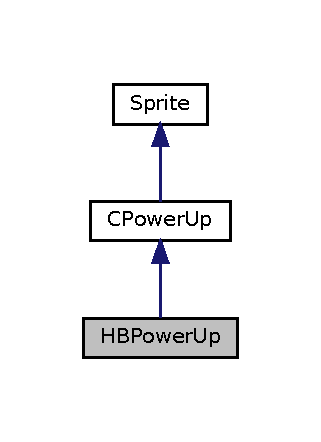
\includegraphics[width=154pt]{classHBPowerUp__inherit__graph}
\end{center}
\end{figure}


Collaboration diagram for H\+B\+Power\+Up\+:\nopagebreak
\begin{figure}[H]
\begin{center}
\leavevmode
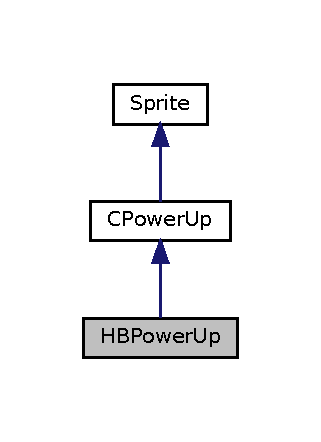
\includegraphics[width=154pt]{classHBPowerUp__coll__graph}
\end{center}
\end{figure}
\subsection*{Public Member Functions}
\begin{DoxyCompactItemize}
\item 
\hyperlink{classHBPowerUp_aa42f5cc3d894cbf0809d22c0f9f9926f}{H\+B\+Power\+Up} (const int pos\+\_\+x, const int pos\+\_\+y)
\item 
\hyperlink{classHBPowerUp_aa6eb33145fcb0f2c8ed0f9a43694aef4}{$\sim$\+H\+B\+Power\+Up} ()
\begin{DoxyCompactList}\small\item\em Default destructor. \end{DoxyCompactList}\item 
void \hyperlink{classHBPowerUp_ac9fcb7d3ef5f3a0561ffe0b6689944a1}{draw} (const int timer)
\end{DoxyCompactItemize}
\subsection*{Additional Inherited Members}


\subsection{Constructor \& Destructor Documentation}
\mbox{\Hypertarget{classHBPowerUp_aa42f5cc3d894cbf0809d22c0f9f9926f}\label{classHBPowerUp_aa42f5cc3d894cbf0809d22c0f9f9926f}} 
\index{H\+B\+Power\+Up@{H\+B\+Power\+Up}!H\+B\+Power\+Up@{H\+B\+Power\+Up}}
\index{H\+B\+Power\+Up@{H\+B\+Power\+Up}!H\+B\+Power\+Up@{H\+B\+Power\+Up}}
\subsubsection{\texorpdfstring{H\+B\+Power\+Up()}{HBPowerUp()}}
{\footnotesize\ttfamily H\+B\+Power\+Up\+::\+H\+B\+Power\+Up (\begin{DoxyParamCaption}\item[{const int}]{pos\+\_\+x,  }\item[{const int}]{pos\+\_\+y }\end{DoxyParamCaption})}

Creates a new instance of a Huge-\/\+Bullet power-\/up and sets it\textquotesingle{}s own index.


\begin{DoxyParams}{Parameters}
{\em pos\+\_\+x} & Point on the X axis where the power-\/up should be placed \\
\hline
{\em pos\+\_\+y} & Point on the Y axis where the power-\/up should be placed \\
\hline
\end{DoxyParams}
\mbox{\Hypertarget{classHBPowerUp_aa6eb33145fcb0f2c8ed0f9a43694aef4}\label{classHBPowerUp_aa6eb33145fcb0f2c8ed0f9a43694aef4}} 
\index{H\+B\+Power\+Up@{H\+B\+Power\+Up}!````~H\+B\+Power\+Up@{$\sim$\+H\+B\+Power\+Up}}
\index{````~H\+B\+Power\+Up@{$\sim$\+H\+B\+Power\+Up}!H\+B\+Power\+Up@{H\+B\+Power\+Up}}
\subsubsection{\texorpdfstring{$\sim$\+H\+B\+Power\+Up()}{~HBPowerUp()}}
{\footnotesize\ttfamily H\+B\+Power\+Up\+::$\sim$\+H\+B\+Power\+Up (\begin{DoxyParamCaption}{ }\end{DoxyParamCaption})}



Default destructor. 



\subsection{Member Function Documentation}
\mbox{\Hypertarget{classHBPowerUp_ac9fcb7d3ef5f3a0561ffe0b6689944a1}\label{classHBPowerUp_ac9fcb7d3ef5f3a0561ffe0b6689944a1}} 
\index{H\+B\+Power\+Up@{H\+B\+Power\+Up}!draw@{draw}}
\index{draw@{draw}!H\+B\+Power\+Up@{H\+B\+Power\+Up}}
\subsubsection{\texorpdfstring{draw()}{draw()}}
{\footnotesize\ttfamily void H\+B\+Power\+Up\+::draw (\begin{DoxyParamCaption}\item[{const int}]{timer }\end{DoxyParamCaption})\hspace{0.3cm}{\ttfamily [virtual]}}

Draws itself on the standard screen. It\textquotesingle{}s overriden because of the different hardcoded color and character it uses as identification.


\begin{DoxyParams}{Parameters}
{\em timer} & Current state of the game\textquotesingle{}s timer. \\
\hline
\end{DoxyParams}


Reimplemented from \hyperlink{classCPowerUp_af1e0bad769efcde21858144596212e01}{C\+Power\+Up}.



The documentation for this class was generated from the following files\+:\begin{DoxyCompactItemize}
\item 
\hyperlink{power__ups_8h}{power\+\_\+ups.\+h}\item 
\hyperlink{power__ups_8cpp}{power\+\_\+ups.\+cpp}\end{DoxyCompactItemize}

\hypertarget{classHugeBullet}{}\section{Huge\+Bullet Class Reference}
\label{classHugeBullet}\index{Huge\+Bullet@{Huge\+Bullet}}


{\ttfamily \#include $<$bullet\+\_\+huge.\+h$>$}



Inheritance diagram for Huge\+Bullet\+:\nopagebreak
\begin{figure}[H]
\begin{center}
\leavevmode
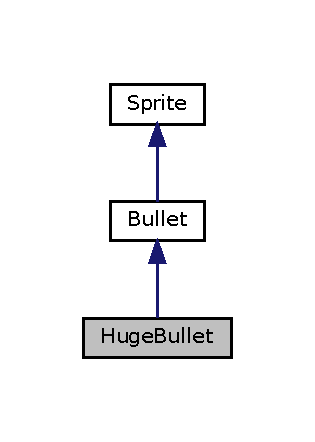
\includegraphics[width=151pt]{classHugeBullet__inherit__graph}
\end{center}
\end{figure}


Collaboration diagram for Huge\+Bullet\+:\nopagebreak
\begin{figure}[H]
\begin{center}
\leavevmode
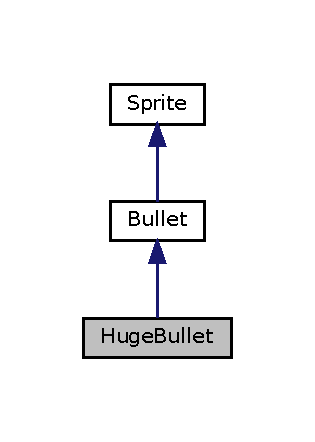
\includegraphics[width=151pt]{classHugeBullet__coll__graph}
\end{center}
\end{figure}
\subsection*{Public Member Functions}
\begin{DoxyCompactItemize}
\item 
\hyperlink{classHugeBullet_a5a486a2079e6e7bd9d97bd40c68c5f85}{Huge\+Bullet} (const int beg\+\_\+x, const int beg\+\_\+y, const int mom\+\_\+x=0, const int mom\+\_\+y=-\/1)
\item 
\hyperlink{classHugeBullet_abdd0ba93e0edc39a7ad94a7f5f38a138}{$\sim$\+Huge\+Bullet} ()
\begin{DoxyCompactList}\small\item\em Default destructor. \end{DoxyCompactList}\item 
bool \hyperlink{classHugeBullet_a6a617486739894eacb79711c8a24bb9d}{overlaps\+With} (\hyperlink{classSprite}{Sprite} $\ast$other\+\_\+sprite) const
\item 
void \hyperlink{classHugeBullet_a0c4f11d7d892b683ecf601cdc37c6ebf}{draw} (const int timer)
\end{DoxyCompactItemize}
\subsection*{Additional Inherited Members}


\subsection{Detailed Description}
This class serves purpose of being the default bullet for \hyperlink{classHBPowerUp}{H\+B\+Power\+Up}. Compared to basic \hyperlink{classBullet}{Bullet}, it is increased in size by a factor of three. 

\subsection{Constructor \& Destructor Documentation}
\mbox{\Hypertarget{classHugeBullet_a5a486a2079e6e7bd9d97bd40c68c5f85}\label{classHugeBullet_a5a486a2079e6e7bd9d97bd40c68c5f85}} 
\index{Huge\+Bullet@{Huge\+Bullet}!Huge\+Bullet@{Huge\+Bullet}}
\index{Huge\+Bullet@{Huge\+Bullet}!Huge\+Bullet@{Huge\+Bullet}}
\subsubsection{\texorpdfstring{Huge\+Bullet()}{HugeBullet()}}
{\footnotesize\ttfamily Huge\+Bullet\+::\+Huge\+Bullet (\begin{DoxyParamCaption}\item[{const int}]{beg\+\_\+x,  }\item[{const int}]{beg\+\_\+y,  }\item[{const int}]{mom\+\_\+x = {\ttfamily 0},  }\item[{const int}]{mom\+\_\+y = {\ttfamily -\/1} }\end{DoxyParamCaption})}

Creates a new instance of a large sized bullet \begin{DoxyNote}{Note}
Compared to \hyperlink{classBullet}{Bullet}, it doesn\textquotesingle{}t use a visual\+\_\+string parameter as it is hardcoded into the class.
\end{DoxyNote}

\begin{DoxyParams}{Parameters}
{\em beg\+\_\+x} & Starting point on X axis for the bullet \\
\hline
{\em beg\+\_\+y} & Starting point on Y axis for the bullet \\
\hline
{\em mom\+\_\+x} & Momentum of the bullet on X axis \\
\hline
{\em mom\+\_\+y} & Momentum of the bullet on Y axis \\
\hline
\end{DoxyParams}
\mbox{\Hypertarget{classHugeBullet_abdd0ba93e0edc39a7ad94a7f5f38a138}\label{classHugeBullet_abdd0ba93e0edc39a7ad94a7f5f38a138}} 
\index{Huge\+Bullet@{Huge\+Bullet}!````~Huge\+Bullet@{$\sim$\+Huge\+Bullet}}
\index{````~Huge\+Bullet@{$\sim$\+Huge\+Bullet}!Huge\+Bullet@{Huge\+Bullet}}
\subsubsection{\texorpdfstring{$\sim$\+Huge\+Bullet()}{~HugeBullet()}}
{\footnotesize\ttfamily Huge\+Bullet\+::$\sim$\+Huge\+Bullet (\begin{DoxyParamCaption}{ }\end{DoxyParamCaption})}



Default destructor. 



\subsection{Member Function Documentation}
\mbox{\Hypertarget{classHugeBullet_a0c4f11d7d892b683ecf601cdc37c6ebf}\label{classHugeBullet_a0c4f11d7d892b683ecf601cdc37c6ebf}} 
\index{Huge\+Bullet@{Huge\+Bullet}!draw@{draw}}
\index{draw@{draw}!Huge\+Bullet@{Huge\+Bullet}}
\subsubsection{\texorpdfstring{draw()}{draw()}}
{\footnotesize\ttfamily void Huge\+Bullet\+::draw (\begin{DoxyParamCaption}\item[{const int}]{timer }\end{DoxyParamCaption})\hspace{0.3cm}{\ttfamily [virtual]}}

Draws itself onto the standard canvas.


\begin{DoxyParams}{Parameters}
{\em timer} & Current state of the games timer \\
\hline
\end{DoxyParams}


Reimplemented from \hyperlink{classSprite_aa41512617e8a1626bade15cbbdfb3f79}{Sprite}.

\mbox{\Hypertarget{classHugeBullet_a6a617486739894eacb79711c8a24bb9d}\label{classHugeBullet_a6a617486739894eacb79711c8a24bb9d}} 
\index{Huge\+Bullet@{Huge\+Bullet}!overlaps\+With@{overlaps\+With}}
\index{overlaps\+With@{overlaps\+With}!Huge\+Bullet@{Huge\+Bullet}}
\subsubsection{\texorpdfstring{overlaps\+With()}{overlapsWith()}}
{\footnotesize\ttfamily bool Huge\+Bullet\+::overlaps\+With (\begin{DoxyParamCaption}\item[{\hyperlink{classSprite}{Sprite} $\ast$}]{other\+\_\+sprite }\end{DoxyParamCaption}) const\hspace{0.3cm}{\ttfamily [virtual]}}

Checks, whether it doesn\textquotesingle{}t overlap with given coordinates \begin{DoxyNote}{Note}
Yes, it doesn\textquotesingle{}t check overlapping of rectangels but rather only a single block.
\end{DoxyNote}

\begin{DoxyParams}{Parameters}
{\em other\+\_\+sprite} & Different graphical element of whose coordinates we want to compare ourselves with \\
\hline
\end{DoxyParams}
\begin{DoxyReturn}{Returns}
Returns true on found overlap, false otherwise 
\end{DoxyReturn}


Reimplemented from \hyperlink{classSprite_a631928eb8d8fabce4f888c6ed76c0885}{Sprite}.



The documentation for this class was generated from the following files\+:\begin{DoxyCompactItemize}
\item 
\hyperlink{bullet__huge_8h}{bullet\+\_\+huge.\+h}\item 
\hyperlink{bullet__huge_8cpp}{bullet\+\_\+huge.\+cpp}\end{DoxyCompactItemize}

\hypertarget{classPlayer}{}\section{Player Class Reference}
\label{classPlayer}\index{Player@{Player}}


{\ttfamily \#include $<$player.\+h$>$}



Inheritance diagram for Player\+:
\nopagebreak
\begin{figure}[H]
\begin{center}
\leavevmode
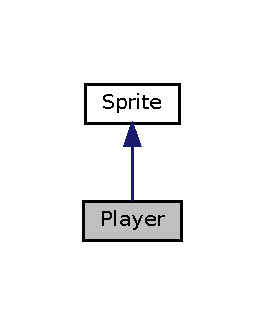
\includegraphics[width=127pt]{classPlayer__inherit__graph}
\end{center}
\end{figure}


Collaboration diagram for Player\+:
\nopagebreak
\begin{figure}[H]
\begin{center}
\leavevmode
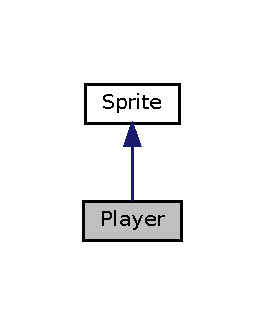
\includegraphics[width=127pt]{classPlayer__coll__graph}
\end{center}
\end{figure}
\subsection*{Public Member Functions}
\begin{DoxyCompactItemize}
\item 
\hyperlink{classPlayer_a7d6d9f5784b5971d9848a9349b6ef377}{Player} (const int beg\+\_\+x=1, const int beg\+\_\+y=1)
\item 
\hyperlink{classPlayer_a749d2c00e1fe0f5c2746f7505a58c062}{$\sim$\+Player} ()
\begin{DoxyCompactList}\small\item\em Default destructor. \end{DoxyCompactList}\item 
void \hyperlink{classPlayer_a5bb630935b83b66406b87149e7087a00}{shoot} (std\+::list$<$ \hyperlink{classSprite}{Sprite} $\ast$$>$ \&bullets\+\_\+ref)
\begin{DoxyCompactList}\small\item\em Makes the rocket shoot using the current shooting method (power-\/up) \end{DoxyCompactList}\item 
void \hyperlink{classPlayer_a856a5c64a431661946ba01b84c969289}{draw} (const int timer)
\item 
void \hyperlink{classPlayer_a52e8800e4216f0d78c497e90412779d2}{set\+Power\+Up} (const int power\+\_\+up\+\_\+index)
\item 
void \hyperlink{classPlayer_a574659d927fef4b34544b728c1631433}{calculate\+New\+Position} (const int timer)
\item 
void \hyperlink{classPlayer_a0646b0f8b1db49816338d0be18175fbe}{handle\+Window\+Collision} (const int screen\+\_\+width, const int screen\+\_\+height)
\end{DoxyCompactItemize}
\subsection*{Public Attributes}
\begin{DoxyCompactItemize}
\item 
double \hyperlink{classPlayer_ad688128863db33f5e527d7e434f557d7}{speedX}
\begin{DoxyCompactList}\small\item\em Speed of the rocket on X axis. \end{DoxyCompactList}\item 
double \hyperlink{classPlayer_abf2d9f3b437bda111c089c01e4b03017}{speedY}
\begin{DoxyCompactList}\small\item\em Speed of the rocket on Y axis. \end{DoxyCompactList}\end{DoxyCompactItemize}
\subsection*{Private Attributes}
\begin{DoxyCompactItemize}
\item 
int \hyperlink{classPlayer_ad7c3f7dc92bc22846e2af9c29eadc3c7}{power\+\_\+up}
\begin{DoxyCompactList}\small\item\em Index of the currently used power-\/up (method of shooting) \end{DoxyCompactList}\item 
double \hyperlink{classPlayer_ae60c030f7922b4c385af29e04c040ccc}{m\+\_\+drag}
\begin{DoxyCompactList}\small\item\em Drag which is applied on every frame. \end{DoxyCompactList}\end{DoxyCompactItemize}
\subsection*{Additional Inherited Members}


\subsection{Detailed Description}
This class serves purpose of being the main player type. Inherits a lot from it\textquotesingle{}s parent class -\/ \hyperlink{classSprite}{Sprite}, but compared to the other \hyperlink{classSprite}{Sprite}\textquotesingle{}s children, it features it\textquotesingle{}s own (simplified) physics engine. 

\subsection{Constructor \& Destructor Documentation}
\mbox{\Hypertarget{classPlayer_a7d6d9f5784b5971d9848a9349b6ef377}\label{classPlayer_a7d6d9f5784b5971d9848a9349b6ef377}} 
\index{Player@{Player}!Player@{Player}}
\index{Player@{Player}!Player@{Player}}
\subsubsection{\texorpdfstring{Player()}{Player()}}
{\footnotesize\ttfamily Player\+::\+Player (\begin{DoxyParamCaption}\item[{const int}]{beg\+\_\+x = {\ttfamily 1},  }\item[{const int}]{beg\+\_\+y = {\ttfamily 1} }\end{DoxyParamCaption})}

Creates a new instance of the player. It sets up m\+\_\+drag to a hardcoded value and resets index of current power-\/up.


\begin{DoxyParams}{Parameters}
{\em beg\+\_\+x} & Starting point on X axis for the player \\
\hline
{\em beg\+\_\+y} & Starting point on Y axis for the player \\
\hline
\end{DoxyParams}
\mbox{\Hypertarget{classPlayer_a749d2c00e1fe0f5c2746f7505a58c062}\label{classPlayer_a749d2c00e1fe0f5c2746f7505a58c062}} 
\index{Player@{Player}!````~Player@{$\sim$\+Player}}
\index{````~Player@{$\sim$\+Player}!Player@{Player}}
\subsubsection{\texorpdfstring{$\sim$\+Player()}{~Player()}}
{\footnotesize\ttfamily Player\+::$\sim$\+Player (\begin{DoxyParamCaption}{ }\end{DoxyParamCaption})}



Default destructor. 



\subsection{Member Function Documentation}
\mbox{\Hypertarget{classPlayer_a574659d927fef4b34544b728c1631433}\label{classPlayer_a574659d927fef4b34544b728c1631433}} 
\index{Player@{Player}!calculate\+New\+Position@{calculate\+New\+Position}}
\index{calculate\+New\+Position@{calculate\+New\+Position}!Player@{Player}}
\subsubsection{\texorpdfstring{calculate\+New\+Position()}{calculateNewPosition()}}
{\footnotesize\ttfamily void Player\+::calculate\+New\+Position (\begin{DoxyParamCaption}\item[{const int}]{timer }\end{DoxyParamCaption})\hspace{0.3cm}{\ttfamily [virtual]}}

Overrides parent\textquotesingle{}s calculatoin method because of it\textquotesingle{}s own movement mechanics. Uses speed, current position and drag to calculate it\textquotesingle{}s new position.


\begin{DoxyParams}{Parameters}
{\em timer} & Current state of the game\textquotesingle{}s timer \\
\hline
\end{DoxyParams}


Reimplemented from \hyperlink{classSprite_a280f80ec30e7d237e3d1380dab27dd31}{Sprite}.

\mbox{\Hypertarget{classPlayer_a856a5c64a431661946ba01b84c969289}\label{classPlayer_a856a5c64a431661946ba01b84c969289}} 
\index{Player@{Player}!draw@{draw}}
\index{draw@{draw}!Player@{Player}}
\subsubsection{\texorpdfstring{draw()}{draw()}}
{\footnotesize\ttfamily void Player\+::draw (\begin{DoxyParamCaption}\item[{const int}]{timer }\end{DoxyParamCaption})\hspace{0.3cm}{\ttfamily [virtual]}}

Overrides parent\textquotesingle{}s drawign function because of it\textquotesingle{}s specific shape.


\begin{DoxyParams}{Parameters}
{\em timer} & Current state of the game\textquotesingle{}s timer \\
\hline
\end{DoxyParams}


Reimplemented from \hyperlink{classSprite_aa41512617e8a1626bade15cbbdfb3f79}{Sprite}.

\mbox{\Hypertarget{classPlayer_a0646b0f8b1db49816338d0be18175fbe}\label{classPlayer_a0646b0f8b1db49816338d0be18175fbe}} 
\index{Player@{Player}!handle\+Window\+Collision@{handle\+Window\+Collision}}
\index{handle\+Window\+Collision@{handle\+Window\+Collision}!Player@{Player}}
\subsubsection{\texorpdfstring{handle\+Window\+Collision()}{handleWindowCollision()}}
{\footnotesize\ttfamily void Player\+::handle\+Window\+Collision (\begin{DoxyParamCaption}\item[{const int}]{screen\+\_\+width,  }\item[{const int}]{screen\+\_\+height }\end{DoxyParamCaption})\hspace{0.3cm}{\ttfamily [virtual]}}

Stops the player from going out of window


\begin{DoxyParams}{Parameters}
{\em screen\+\_\+width} & Current width of the screen in character blocks \\
\hline
{\em screen\+\_\+height} & Current height of the screen in character blocks \\
\hline
\end{DoxyParams}


Reimplemented from \hyperlink{classSprite_a88935cd050a81898ee3a5693038f1a7a}{Sprite}.

\mbox{\Hypertarget{classPlayer_a52e8800e4216f0d78c497e90412779d2}\label{classPlayer_a52e8800e4216f0d78c497e90412779d2}} 
\index{Player@{Player}!set\+Power\+Up@{set\+Power\+Up}}
\index{set\+Power\+Up@{set\+Power\+Up}!Player@{Player}}
\subsubsection{\texorpdfstring{set\+Power\+Up()}{setPowerUp()}}
{\footnotesize\ttfamily void Player\+::set\+Power\+Up (\begin{DoxyParamCaption}\item[{const int}]{power\+\_\+up\+\_\+index }\end{DoxyParamCaption})}

Setter for the player\textquotesingle{}s shooting method (index of the power-\/up)


\begin{DoxyParams}{Parameters}
{\em power\+\_\+up\+\_\+index} & New shooting method \\
\hline
\end{DoxyParams}
\mbox{\Hypertarget{classPlayer_a5bb630935b83b66406b87149e7087a00}\label{classPlayer_a5bb630935b83b66406b87149e7087a00}} 
\index{Player@{Player}!shoot@{shoot}}
\index{shoot@{shoot}!Player@{Player}}
\subsubsection{\texorpdfstring{shoot()}{shoot()}}
{\footnotesize\ttfamily void Player\+::shoot (\begin{DoxyParamCaption}\item[{std\+::list$<$ \hyperlink{classSprite}{Sprite} $\ast$$>$ \&}]{bullets\+\_\+ref }\end{DoxyParamCaption})}



Makes the rocket shoot using the current shooting method (power-\/up) 

Checks the current shooting method and adds a bullet to the game\textquotesingle{}s bullet list accordingly.


\begin{DoxyParams}{Parameters}
{\em bullets\+\_\+ref} & Reference to the game\textquotesingle{}s list with bullets \\
\hline
\end{DoxyParams}


\subsection{Member Data Documentation}
\mbox{\Hypertarget{classPlayer_ae60c030f7922b4c385af29e04c040ccc}\label{classPlayer_ae60c030f7922b4c385af29e04c040ccc}} 
\index{Player@{Player}!m\+\_\+drag@{m\+\_\+drag}}
\index{m\+\_\+drag@{m\+\_\+drag}!Player@{Player}}
\subsubsection{\texorpdfstring{m\+\_\+drag}{m\_drag}}
{\footnotesize\ttfamily double Player\+::m\+\_\+drag\hspace{0.3cm}{\ttfamily [private]}}



Drag which is applied on every frame. 

\mbox{\Hypertarget{classPlayer_ad7c3f7dc92bc22846e2af9c29eadc3c7}\label{classPlayer_ad7c3f7dc92bc22846e2af9c29eadc3c7}} 
\index{Player@{Player}!power\+\_\+up@{power\+\_\+up}}
\index{power\+\_\+up@{power\+\_\+up}!Player@{Player}}
\subsubsection{\texorpdfstring{power\+\_\+up}{power\_up}}
{\footnotesize\ttfamily int Player\+::power\+\_\+up\hspace{0.3cm}{\ttfamily [private]}}



Index of the currently used power-\/up (method of shooting) 

\mbox{\Hypertarget{classPlayer_ad688128863db33f5e527d7e434f557d7}\label{classPlayer_ad688128863db33f5e527d7e434f557d7}} 
\index{Player@{Player}!speedX@{speedX}}
\index{speedX@{speedX}!Player@{Player}}
\subsubsection{\texorpdfstring{speedX}{speedX}}
{\footnotesize\ttfamily double Player\+::speedX}



Speed of the rocket on X axis. 

\mbox{\Hypertarget{classPlayer_abf2d9f3b437bda111c089c01e4b03017}\label{classPlayer_abf2d9f3b437bda111c089c01e4b03017}} 
\index{Player@{Player}!speedY@{speedY}}
\index{speedY@{speedY}!Player@{Player}}
\subsubsection{\texorpdfstring{speedY}{speedY}}
{\footnotesize\ttfamily double Player\+::speedY}



Speed of the rocket on Y axis. 



The documentation for this class was generated from the following files\+:\begin{DoxyCompactItemize}
\item 
\hyperlink{player_8h}{player.\+h}\item 
\hyperlink{player_8cpp}{player.\+cpp}\end{DoxyCompactItemize}

\hypertarget{classSprite}{}\section{Sprite Class Reference}
\label{classSprite}\index{Sprite@{Sprite}}


{\ttfamily \#include $<$sprite.\+h$>$}



Inheritance diagram for Sprite\+:\nopagebreak
\begin{figure}[H]
\begin{center}
\leavevmode
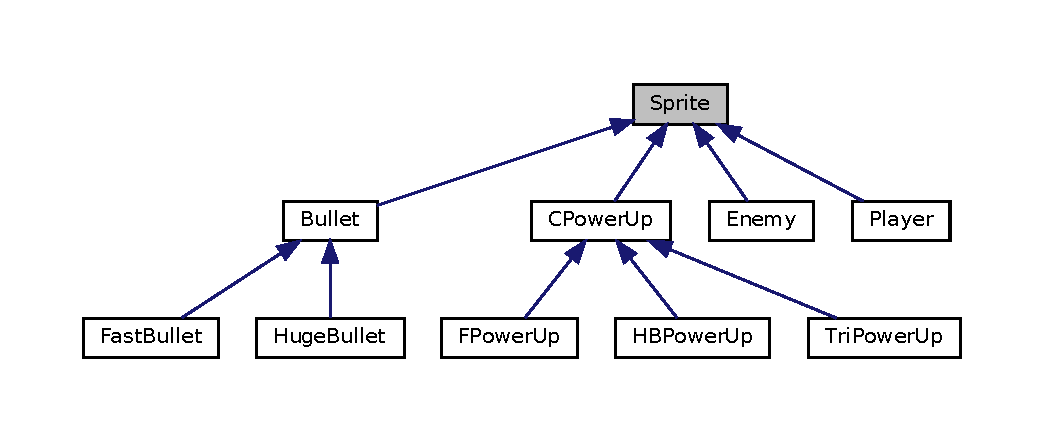
\includegraphics[width=350pt]{classSprite__inherit__graph}
\end{center}
\end{figure}
\subsection*{Public Member Functions}
\begin{DoxyCompactItemize}
\item 
\hyperlink{classSprite_aa9bd46689aaa0c9d5cf102fa153c8554}{Sprite} (const char $\ast$visual\+\_\+string, const int beg\+\_\+x=0, const int beg\+\_\+y=0)
\item 
virtual \hyperlink{classSprite_a8accab430f9d90ae5117b57d67e32b84}{$\sim$\+Sprite} ()
\begin{DoxyCompactList}\small\item\em Default destructor. \end{DoxyCompactList}\item 
virtual void \hyperlink{classSprite_a280f80ec30e7d237e3d1380dab27dd31}{calculate\+New\+Position} (const int timer)
\item 
bool \hyperlink{classSprite_a47ac98fad52841eb22a62f6854f66e1f}{get\+Visibility} () const
\item 
void \hyperlink{classSprite_ac0df5147803b139aa433b33eb2a42246}{set\+Visibility} (const bool new\+\_\+visibility)
\item 
int \hyperlink{classSprite_aad0915304f3b279846eb9868c6651d1a}{positionX} () const
\item 
int \hyperlink{classSprite_a58b317b273657123c3050114d5e50d1b}{positionY} () const
\item 
virtual bool \hyperlink{classSprite_a631928eb8d8fabce4f888c6ed76c0885}{overlaps\+With} (\hyperlink{classSprite}{Sprite} $\ast$other\+\_\+sprite) const
\item 
virtual void \hyperlink{classSprite_aa41512617e8a1626bade15cbbdfb3f79}{draw} (const int timer)
\item 
virtual void \hyperlink{classSprite_a88935cd050a81898ee3a5693038f1a7a}{handle\+Window\+Collision} (const int screen\+\_\+width, const int screen\+\_\+height)
\end{DoxyCompactItemize}
\subsection*{Protected Attributes}
\begin{DoxyCompactItemize}
\item 
const char $\ast$ \hyperlink{classSprite_adf82741e0c96c05cdd1c96ceda8df837}{m\+\_\+visual\+\_\+string}
\begin{DoxyCompactList}\small\item\em String of characters representing the sprite on the screen. \end{DoxyCompactList}\item 
bool \hyperlink{classSprite_ad0254af9247c4e1d5d220bb89b3ef745}{m\+\_\+visible}
\item 
int \hyperlink{classSprite_adf17b6ade9cc7dffc1833bc6649b6a13}{m\+\_\+update\+\_\+freq}
\begin{DoxyCompactList}\small\item\em Basically stores a position in timer, when the position of the sprite shall be recalculated. \end{DoxyCompactList}\item 
double \hyperlink{classSprite_ac0a1a6a0c8fce6f46b30152b263fd2a9}{m\+\_\+x}
\begin{DoxyCompactList}\small\item\em Position on the X axis of the screen for the sprite. \end{DoxyCompactList}\item 
double \hyperlink{classSprite_adc245ad211b04b31cd234fb080b4b034}{m\+\_\+y}
\begin{DoxyCompactList}\small\item\em Position on the Y axis of the screen for the sprite. \end{DoxyCompactList}\item 
int \hyperlink{classSprite_ada1b4009e13a72b62fc139bb5f182a12}{m\+\_\+direction\+\_\+x}
\begin{DoxyCompactList}\small\item\em Basically momentum of the sprite on the X axis. \end{DoxyCompactList}\item 
int \hyperlink{classSprite_ab55aaafbb990f7d5c6f93b513dd5ce62}{m\+\_\+direction\+\_\+y}
\begin{DoxyCompactList}\small\item\em Basically momentum of the sprite on the Y axis. \end{DoxyCompactList}\end{DoxyCompactItemize}


\subsection{Detailed Description}
Our main parent class for all of the graphical objects. 

\subsection{Constructor \& Destructor Documentation}
\mbox{\Hypertarget{classSprite_aa9bd46689aaa0c9d5cf102fa153c8554}\label{classSprite_aa9bd46689aaa0c9d5cf102fa153c8554}} 
\index{Sprite@{Sprite}!Sprite@{Sprite}}
\index{Sprite@{Sprite}!Sprite@{Sprite}}
\subsubsection{\texorpdfstring{Sprite()}{Sprite()}}
{\footnotesize\ttfamily Sprite\+::\+Sprite (\begin{DoxyParamCaption}\item[{const char $\ast$}]{visual\+\_\+string,  }\item[{const int}]{beg\+\_\+x = {\ttfamily 0},  }\item[{const int}]{beg\+\_\+y = {\ttfamily 0} }\end{DoxyParamCaption})}

Creates a new instance of a basic sprite type

update\+\_\+frequency is set to zero visible is set to true


\begin{DoxyParams}{Parameters}
{\em visual\+\_\+string} & String of characters which represents the sprite on the screen. \\
\hline
{\em beg\+\_\+x} & Starting point on X axis for the bullet \\
\hline
{\em beg\+\_\+y} & Starting point on Y axis for the bullet \\
\hline
\end{DoxyParams}
\mbox{\Hypertarget{classSprite_a8accab430f9d90ae5117b57d67e32b84}\label{classSprite_a8accab430f9d90ae5117b57d67e32b84}} 
\index{Sprite@{Sprite}!````~Sprite@{$\sim$\+Sprite}}
\index{````~Sprite@{$\sim$\+Sprite}!Sprite@{Sprite}}
\subsubsection{\texorpdfstring{$\sim$\+Sprite()}{~Sprite()}}
{\footnotesize\ttfamily Sprite\+::$\sim$\+Sprite (\begin{DoxyParamCaption}{ }\end{DoxyParamCaption})\hspace{0.3cm}{\ttfamily [virtual]}}



Default destructor. 



\subsection{Member Function Documentation}
\mbox{\Hypertarget{classSprite_a280f80ec30e7d237e3d1380dab27dd31}\label{classSprite_a280f80ec30e7d237e3d1380dab27dd31}} 
\index{Sprite@{Sprite}!calculate\+New\+Position@{calculate\+New\+Position}}
\index{calculate\+New\+Position@{calculate\+New\+Position}!Sprite@{Sprite}}
\subsubsection{\texorpdfstring{calculate\+New\+Position()}{calculateNewPosition()}}
{\footnotesize\ttfamily void Sprite\+::calculate\+New\+Position (\begin{DoxyParamCaption}\item[{const int}]{timer }\end{DoxyParamCaption})\hspace{0.3cm}{\ttfamily [virtual]}}

Recalculates the current position based on the m\+\_\+direction and current state of the game\textquotesingle{}s timer


\begin{DoxyParams}{Parameters}
{\em timer} & Current state of the game\textquotesingle{}s timer \\
\hline
\end{DoxyParams}


Reimplemented in \hyperlink{classPlayer_a574659d927fef4b34544b728c1631433}{Player}.

\mbox{\Hypertarget{classSprite_aa41512617e8a1626bade15cbbdfb3f79}\label{classSprite_aa41512617e8a1626bade15cbbdfb3f79}} 
\index{Sprite@{Sprite}!draw@{draw}}
\index{draw@{draw}!Sprite@{Sprite}}
\subsubsection{\texorpdfstring{draw()}{draw()}}
{\footnotesize\ttfamily void Sprite\+::draw (\begin{DoxyParamCaption}\item[{const int}]{timer }\end{DoxyParamCaption})\hspace{0.3cm}{\ttfamily [virtual]}}

Draws itself onto the standard canvas.


\begin{DoxyParams}{Parameters}
{\em timer} & Current state of the games timer \\
\hline
\end{DoxyParams}


Reimplemented in \hyperlink{classFPowerUp_aaf83782b032f53dacd37650127595148}{F\+Power\+Up}, \hyperlink{classHBPowerUp_ac9fcb7d3ef5f3a0561ffe0b6689944a1}{H\+B\+Power\+Up}, \hyperlink{classTriPowerUp_a06af18b739589c56a90da91716243acf}{Tri\+Power\+Up}, \hyperlink{classPlayer_a856a5c64a431661946ba01b84c969289}{Player}, \hyperlink{classCPowerUp_af1e0bad769efcde21858144596212e01}{C\+Power\+Up}, and \hyperlink{classHugeBullet_a0c4f11d7d892b683ecf601cdc37c6ebf}{Huge\+Bullet}.

\mbox{\Hypertarget{classSprite_a47ac98fad52841eb22a62f6854f66e1f}\label{classSprite_a47ac98fad52841eb22a62f6854f66e1f}} 
\index{Sprite@{Sprite}!get\+Visibility@{get\+Visibility}}
\index{get\+Visibility@{get\+Visibility}!Sprite@{Sprite}}
\subsubsection{\texorpdfstring{get\+Visibility()}{getVisibility()}}
{\footnotesize\ttfamily bool Sprite\+::get\+Visibility (\begin{DoxyParamCaption}{ }\end{DoxyParamCaption}) const}

Returns current visibilty of the sprite

\begin{DoxyReturn}{Returns}
Returns true if the sprite is visible, otherwise returns false 
\end{DoxyReturn}
\mbox{\Hypertarget{classSprite_a88935cd050a81898ee3a5693038f1a7a}\label{classSprite_a88935cd050a81898ee3a5693038f1a7a}} 
\index{Sprite@{Sprite}!handle\+Window\+Collision@{handle\+Window\+Collision}}
\index{handle\+Window\+Collision@{handle\+Window\+Collision}!Sprite@{Sprite}}
\subsubsection{\texorpdfstring{handle\+Window\+Collision()}{handleWindowCollision()}}
{\footnotesize\ttfamily void Sprite\+::handle\+Window\+Collision (\begin{DoxyParamCaption}\item[{const int}]{screen\+\_\+width,  }\item[{const int}]{screen\+\_\+height }\end{DoxyParamCaption})\hspace{0.3cm}{\ttfamily [virtual]}}

Function to check, whether the sprite got out of the viewport. If so, it sets it\textquotesingle{}s visibility to false


\begin{DoxyParams}{Parameters}
{\em screen\+\_\+width} & Current width of the screen in character blocks \\
\hline
{\em screen\+\_\+height} & Current height of the screen in character blocks \\
\hline
\end{DoxyParams}


Reimplemented in \hyperlink{classPlayer_a0646b0f8b1db49816338d0be18175fbe}{Player}.

\mbox{\Hypertarget{classSprite_a631928eb8d8fabce4f888c6ed76c0885}\label{classSprite_a631928eb8d8fabce4f888c6ed76c0885}} 
\index{Sprite@{Sprite}!overlaps\+With@{overlaps\+With}}
\index{overlaps\+With@{overlaps\+With}!Sprite@{Sprite}}
\subsubsection{\texorpdfstring{overlaps\+With()}{overlapsWith()}}
{\footnotesize\ttfamily bool Sprite\+::overlaps\+With (\begin{DoxyParamCaption}\item[{\hyperlink{classSprite}{Sprite} $\ast$}]{other\+\_\+sprite }\end{DoxyParamCaption}) const\hspace{0.3cm}{\ttfamily [virtual]}}

Checks, whether it doesn\textquotesingle{}t overlap with given coordinates \begin{DoxyNote}{Note}
Yes, it doesn\textquotesingle{}t check overlapping of rectangels but rather only a single block.
\end{DoxyNote}

\begin{DoxyParams}{Parameters}
{\em other\+\_\+sprite} & Different graphical element of whose coordinates we want to compare ourselves with \\
\hline
\end{DoxyParams}
\begin{DoxyReturn}{Returns}
Returns true on found overlap, false otherwise 
\end{DoxyReturn}


Reimplemented in \hyperlink{classHugeBullet_a6a617486739894eacb79711c8a24bb9d}{Huge\+Bullet}.

\mbox{\Hypertarget{classSprite_aad0915304f3b279846eb9868c6651d1a}\label{classSprite_aad0915304f3b279846eb9868c6651d1a}} 
\index{Sprite@{Sprite}!positionX@{positionX}}
\index{positionX@{positionX}!Sprite@{Sprite}}
\subsubsection{\texorpdfstring{position\+X()}{positionX()}}
{\footnotesize\ttfamily int Sprite\+::positionX (\begin{DoxyParamCaption}{ }\end{DoxyParamCaption}) const}

Returns current position on the screen\textquotesingle{}s X axis of the sprite

\begin{DoxyReturn}{Returns}
current position on the screen\textquotesingle{}s X axis of the sprite 
\end{DoxyReturn}
\mbox{\Hypertarget{classSprite_a58b317b273657123c3050114d5e50d1b}\label{classSprite_a58b317b273657123c3050114d5e50d1b}} 
\index{Sprite@{Sprite}!positionY@{positionY}}
\index{positionY@{positionY}!Sprite@{Sprite}}
\subsubsection{\texorpdfstring{position\+Y()}{positionY()}}
{\footnotesize\ttfamily int Sprite\+::positionY (\begin{DoxyParamCaption}{ }\end{DoxyParamCaption}) const}

Returns current position on the screen\textquotesingle{}s Y axis of the sprite

\begin{DoxyReturn}{Returns}
current position on the screen\textquotesingle{}s Y axis of the sprite 
\end{DoxyReturn}
\mbox{\Hypertarget{classSprite_ac0df5147803b139aa433b33eb2a42246}\label{classSprite_ac0df5147803b139aa433b33eb2a42246}} 
\index{Sprite@{Sprite}!set\+Visibility@{set\+Visibility}}
\index{set\+Visibility@{set\+Visibility}!Sprite@{Sprite}}
\subsubsection{\texorpdfstring{set\+Visibility()}{setVisibility()}}
{\footnotesize\ttfamily void Sprite\+::set\+Visibility (\begin{DoxyParamCaption}\item[{const bool}]{new\+\_\+visibility }\end{DoxyParamCaption})}

Sets a new visibility value


\begin{DoxyParams}{Parameters}
{\em new\+\_\+visibility} & New state of the sprite\textquotesingle{}s visibility \\
\hline
\end{DoxyParams}


\subsection{Member Data Documentation}
\mbox{\Hypertarget{classSprite_ada1b4009e13a72b62fc139bb5f182a12}\label{classSprite_ada1b4009e13a72b62fc139bb5f182a12}} 
\index{Sprite@{Sprite}!m\+\_\+direction\+\_\+x@{m\+\_\+direction\+\_\+x}}
\index{m\+\_\+direction\+\_\+x@{m\+\_\+direction\+\_\+x}!Sprite@{Sprite}}
\subsubsection{\texorpdfstring{m\+\_\+direction\+\_\+x}{m\_direction\_x}}
{\footnotesize\ttfamily int Sprite\+::m\+\_\+direction\+\_\+x\hspace{0.3cm}{\ttfamily [protected]}}



Basically momentum of the sprite on the X axis. 

\mbox{\Hypertarget{classSprite_ab55aaafbb990f7d5c6f93b513dd5ce62}\label{classSprite_ab55aaafbb990f7d5c6f93b513dd5ce62}} 
\index{Sprite@{Sprite}!m\+\_\+direction\+\_\+y@{m\+\_\+direction\+\_\+y}}
\index{m\+\_\+direction\+\_\+y@{m\+\_\+direction\+\_\+y}!Sprite@{Sprite}}
\subsubsection{\texorpdfstring{m\+\_\+direction\+\_\+y}{m\_direction\_y}}
{\footnotesize\ttfamily int Sprite\+::m\+\_\+direction\+\_\+y\hspace{0.3cm}{\ttfamily [protected]}}



Basically momentum of the sprite on the Y axis. 

\mbox{\Hypertarget{classSprite_adf17b6ade9cc7dffc1833bc6649b6a13}\label{classSprite_adf17b6ade9cc7dffc1833bc6649b6a13}} 
\index{Sprite@{Sprite}!m\+\_\+update\+\_\+freq@{m\+\_\+update\+\_\+freq}}
\index{m\+\_\+update\+\_\+freq@{m\+\_\+update\+\_\+freq}!Sprite@{Sprite}}
\subsubsection{\texorpdfstring{m\+\_\+update\+\_\+freq}{m\_update\_freq}}
{\footnotesize\ttfamily int Sprite\+::m\+\_\+update\+\_\+freq\hspace{0.3cm}{\ttfamily [protected]}}



Basically stores a position in timer, when the position of the sprite shall be recalculated. 

\mbox{\Hypertarget{classSprite_ad0254af9247c4e1d5d220bb89b3ef745}\label{classSprite_ad0254af9247c4e1d5d220bb89b3ef745}} 
\index{Sprite@{Sprite}!m\+\_\+visible@{m\+\_\+visible}}
\index{m\+\_\+visible@{m\+\_\+visible}!Sprite@{Sprite}}
\subsubsection{\texorpdfstring{m\+\_\+visible}{m\_visible}}
{\footnotesize\ttfamily bool Sprite\+::m\+\_\+visible\hspace{0.3cm}{\ttfamily [protected]}}

Boolean variable to store sprite\textquotesingle{}s state. In current implementation of the game, any object that becomes invisible, will be destroyed and removed from a list that it\textquotesingle{}s memeber of. \mbox{\Hypertarget{classSprite_adf82741e0c96c05cdd1c96ceda8df837}\label{classSprite_adf82741e0c96c05cdd1c96ceda8df837}} 
\index{Sprite@{Sprite}!m\+\_\+visual\+\_\+string@{m\+\_\+visual\+\_\+string}}
\index{m\+\_\+visual\+\_\+string@{m\+\_\+visual\+\_\+string}!Sprite@{Sprite}}
\subsubsection{\texorpdfstring{m\+\_\+visual\+\_\+string}{m\_visual\_string}}
{\footnotesize\ttfamily const char$\ast$ Sprite\+::m\+\_\+visual\+\_\+string\hspace{0.3cm}{\ttfamily [protected]}}



String of characters representing the sprite on the screen. 

\mbox{\Hypertarget{classSprite_ac0a1a6a0c8fce6f46b30152b263fd2a9}\label{classSprite_ac0a1a6a0c8fce6f46b30152b263fd2a9}} 
\index{Sprite@{Sprite}!m\+\_\+x@{m\+\_\+x}}
\index{m\+\_\+x@{m\+\_\+x}!Sprite@{Sprite}}
\subsubsection{\texorpdfstring{m\+\_\+x}{m\_x}}
{\footnotesize\ttfamily double Sprite\+::m\+\_\+x\hspace{0.3cm}{\ttfamily [protected]}}



Position on the X axis of the screen for the sprite. 

\mbox{\Hypertarget{classSprite_adc245ad211b04b31cd234fb080b4b034}\label{classSprite_adc245ad211b04b31cd234fb080b4b034}} 
\index{Sprite@{Sprite}!m\+\_\+y@{m\+\_\+y}}
\index{m\+\_\+y@{m\+\_\+y}!Sprite@{Sprite}}
\subsubsection{\texorpdfstring{m\+\_\+y}{m\_y}}
{\footnotesize\ttfamily double Sprite\+::m\+\_\+y\hspace{0.3cm}{\ttfamily [protected]}}



Position on the Y axis of the screen for the sprite. 



The documentation for this class was generated from the following files\+:\begin{DoxyCompactItemize}
\item 
\hyperlink{sprite_8h}{sprite.\+h}\item 
\hyperlink{sprite_8cpp}{sprite.\+cpp}\end{DoxyCompactItemize}

\hypertarget{classTriPowerUp}{}\section{Tri\+Power\+Up Class Reference}
\label{classTriPowerUp}\index{Tri\+Power\+Up@{Tri\+Power\+Up}}


{\ttfamily \#include $<$power\+\_\+ups.\+h$>$}



Inheritance diagram for Tri\+Power\+Up\+:\nopagebreak
\begin{figure}[H]
\begin{center}
\leavevmode
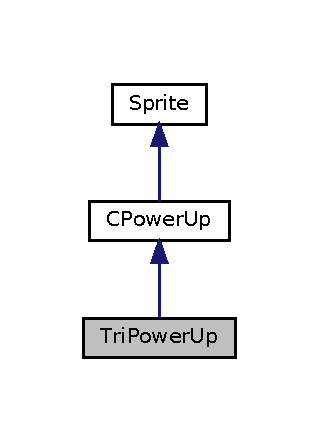
\includegraphics[width=153pt]{classTriPowerUp__inherit__graph}
\end{center}
\end{figure}


Collaboration diagram for Tri\+Power\+Up\+:\nopagebreak
\begin{figure}[H]
\begin{center}
\leavevmode
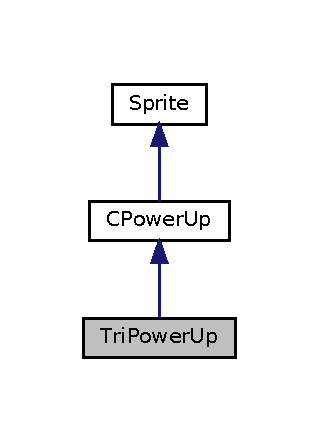
\includegraphics[width=153pt]{classTriPowerUp__coll__graph}
\end{center}
\end{figure}
\subsection*{Public Member Functions}
\begin{DoxyCompactItemize}
\item 
\hyperlink{classTriPowerUp_a67d6278e6c22cf50f3b15763dbb6da88}{Tri\+Power\+Up} (const int pos\+\_\+x, const int pos\+\_\+y)
\item 
\hyperlink{classTriPowerUp_a243237700fae7d620aae0f8d308533f1}{$\sim$\+Tri\+Power\+Up} ()
\begin{DoxyCompactList}\small\item\em Default destructor. \end{DoxyCompactList}\item 
void \hyperlink{classTriPowerUp_a06af18b739589c56a90da91716243acf}{draw} (const int timer)
\end{DoxyCompactItemize}
\subsection*{Additional Inherited Members}


\subsection{Constructor \& Destructor Documentation}
\mbox{\Hypertarget{classTriPowerUp_a67d6278e6c22cf50f3b15763dbb6da88}\label{classTriPowerUp_a67d6278e6c22cf50f3b15763dbb6da88}} 
\index{Tri\+Power\+Up@{Tri\+Power\+Up}!Tri\+Power\+Up@{Tri\+Power\+Up}}
\index{Tri\+Power\+Up@{Tri\+Power\+Up}!Tri\+Power\+Up@{Tri\+Power\+Up}}
\subsubsection{\texorpdfstring{Tri\+Power\+Up()}{TriPowerUp()}}
{\footnotesize\ttfamily Tri\+Power\+Up\+::\+Tri\+Power\+Up (\begin{DoxyParamCaption}\item[{const int}]{pos\+\_\+x,  }\item[{const int}]{pos\+\_\+y }\end{DoxyParamCaption})}

Creates a new instance of a Triple-\/\+Bullet power-\/up and sets it\textquotesingle{}s own index.


\begin{DoxyParams}{Parameters}
{\em pos\+\_\+x} & Point on the X axis where the power-\/up should be placed \\
\hline
{\em pos\+\_\+y} & Point on the Y axis where the power-\/up should be placed \\
\hline
\end{DoxyParams}
\mbox{\Hypertarget{classTriPowerUp_a243237700fae7d620aae0f8d308533f1}\label{classTriPowerUp_a243237700fae7d620aae0f8d308533f1}} 
\index{Tri\+Power\+Up@{Tri\+Power\+Up}!````~Tri\+Power\+Up@{$\sim$\+Tri\+Power\+Up}}
\index{````~Tri\+Power\+Up@{$\sim$\+Tri\+Power\+Up}!Tri\+Power\+Up@{Tri\+Power\+Up}}
\subsubsection{\texorpdfstring{$\sim$\+Tri\+Power\+Up()}{~TriPowerUp()}}
{\footnotesize\ttfamily Tri\+Power\+Up\+::$\sim$\+Tri\+Power\+Up (\begin{DoxyParamCaption}{ }\end{DoxyParamCaption})}



Default destructor. 



\subsection{Member Function Documentation}
\mbox{\Hypertarget{classTriPowerUp_a06af18b739589c56a90da91716243acf}\label{classTriPowerUp_a06af18b739589c56a90da91716243acf}} 
\index{Tri\+Power\+Up@{Tri\+Power\+Up}!draw@{draw}}
\index{draw@{draw}!Tri\+Power\+Up@{Tri\+Power\+Up}}
\subsubsection{\texorpdfstring{draw()}{draw()}}
{\footnotesize\ttfamily void Tri\+Power\+Up\+::draw (\begin{DoxyParamCaption}\item[{const int}]{timer }\end{DoxyParamCaption})\hspace{0.3cm}{\ttfamily [virtual]}}

Draws itself on the standard screen. It\textquotesingle{}s overriden because of the different hardcoded color and character it uses as identification.


\begin{DoxyParams}{Parameters}
{\em timer} & Current state of the game\textquotesingle{}s timer. \\
\hline
\end{DoxyParams}


Reimplemented from \hyperlink{classCPowerUp_af1e0bad769efcde21858144596212e01}{C\+Power\+Up}.



The documentation for this class was generated from the following files\+:\begin{DoxyCompactItemize}
\item 
\hyperlink{power__ups_8h}{power\+\_\+ups.\+h}\item 
\hyperlink{power__ups_8cpp}{power\+\_\+ups.\+cpp}\end{DoxyCompactItemize}

\chapter{File Documentation}
\hypertarget{bullet_8cpp}{}\section{bullet.\+cpp File Reference}
\label{bullet_8cpp}\index{bullet.\+cpp@{bullet.\+cpp}}
{\ttfamily \#include \char`\"{}sprite.\+h\char`\"{}}\newline
{\ttfamily \#include \char`\"{}bullet.\+h\char`\"{}}\newline
Include dependency graph for bullet.\+cpp\+:
\nopagebreak
\begin{figure}[H]
\begin{center}
\leavevmode
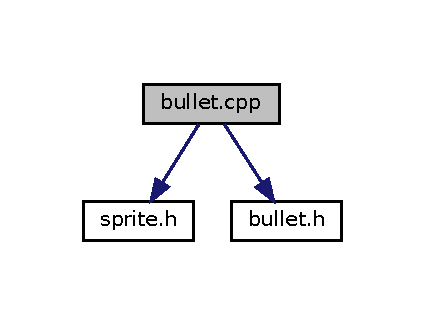
\includegraphics[width=204pt]{bullet_8cpp__incl}
\end{center}
\end{figure}

\hypertarget{bullet_8h}{}\section{bullet.\+h File Reference}
\label{bullet_8h}\index{bullet.\+h@{bullet.\+h}}
This graph shows which files directly or indirectly include this file\+:
\nopagebreak
\begin{figure}[H]
\begin{center}
\leavevmode
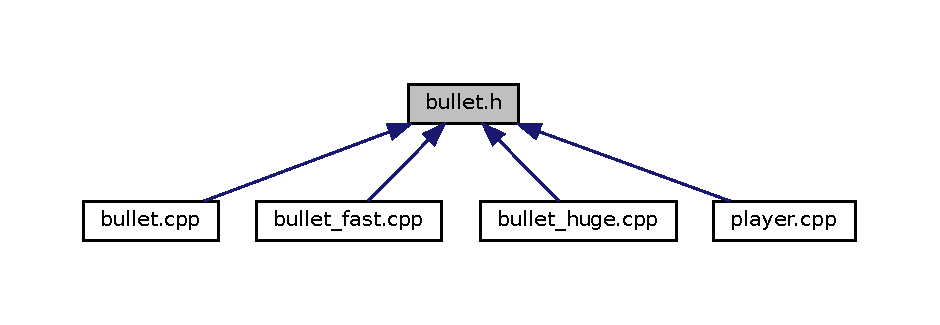
\includegraphics[width=350pt]{bullet_8h__dep__incl}
\end{center}
\end{figure}
\subsection*{Classes}
\begin{DoxyCompactItemize}
\item 
class \hyperlink{classBullet}{Bullet}
\end{DoxyCompactItemize}

\hypertarget{bullet__fast_8cpp}{}\section{bullet\+\_\+fast.\+cpp File Reference}
\label{bullet__fast_8cpp}\index{bullet\+\_\+fast.\+cpp@{bullet\+\_\+fast.\+cpp}}
{\ttfamily \#include \char`\"{}sprite.\+h\char`\"{}}\newline
{\ttfamily \#include \char`\"{}bullet.\+h\char`\"{}}\newline
{\ttfamily \#include \char`\"{}bullet\+\_\+fast.\+h\char`\"{}}\newline
Include dependency graph for bullet\+\_\+fast.\+cpp\+:
\nopagebreak
\begin{figure}[H]
\begin{center}
\leavevmode
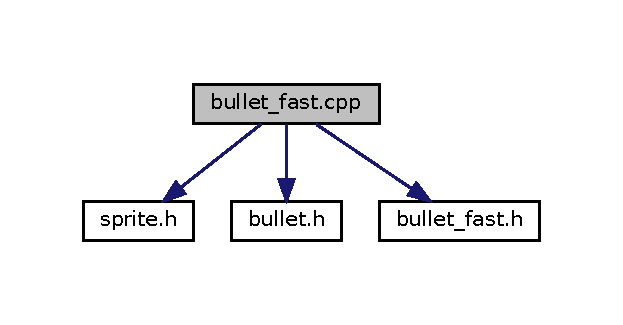
\includegraphics[width=299pt]{bullet__fast_8cpp__incl}
\end{center}
\end{figure}

\hypertarget{bullet__fast_8h}{}\section{bullet\+\_\+fast.\+h File Reference}
\label{bullet__fast_8h}\index{bullet\+\_\+fast.\+h@{bullet\+\_\+fast.\+h}}
This graph shows which files directly or indirectly include this file\+:
\nopagebreak
\begin{figure}[H]
\begin{center}
\leavevmode
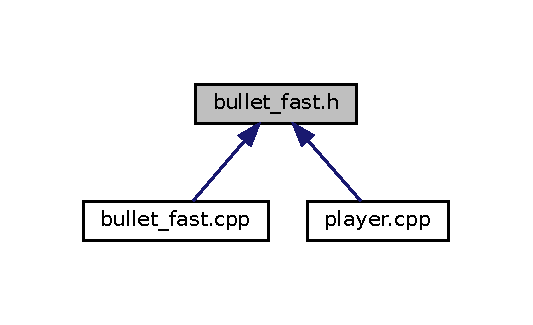
\includegraphics[width=256pt]{bullet__fast_8h__dep__incl}
\end{center}
\end{figure}
\subsection*{Classes}
\begin{DoxyCompactItemize}
\item 
class \hyperlink{classFastBullet}{Fast\+Bullet}
\end{DoxyCompactItemize}

\hypertarget{bullet__huge_8cpp}{}\section{bullet\+\_\+huge.\+cpp File Reference}
\label{bullet__huge_8cpp}\index{bullet\+\_\+huge.\+cpp@{bullet\+\_\+huge.\+cpp}}
{\ttfamily \#include \char`\"{}custom\+\_\+ncurses.\+h\char`\"{}}\newline
{\ttfamily \#include \char`\"{}sprite.\+h\char`\"{}}\newline
{\ttfamily \#include \char`\"{}bullet.\+h\char`\"{}}\newline
{\ttfamily \#include \char`\"{}bullet\+\_\+huge.\+h\char`\"{}}\newline
Include dependency graph for bullet\+\_\+huge.\+cpp\+:\nopagebreak
\begin{figure}[H]
\begin{center}
\leavevmode
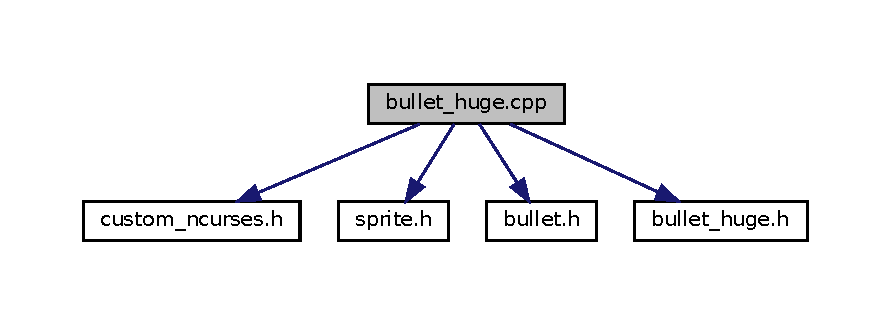
\includegraphics[width=350pt]{bullet__huge_8cpp__incl}
\end{center}
\end{figure}

\hypertarget{bullet__huge_8h}{}\section{bullet\+\_\+huge.\+h File Reference}
\label{bullet__huge_8h}\index{bullet\+\_\+huge.\+h@{bullet\+\_\+huge.\+h}}
This graph shows which files directly or indirectly include this file\+:
\nopagebreak
\begin{figure}[H]
\begin{center}
\leavevmode
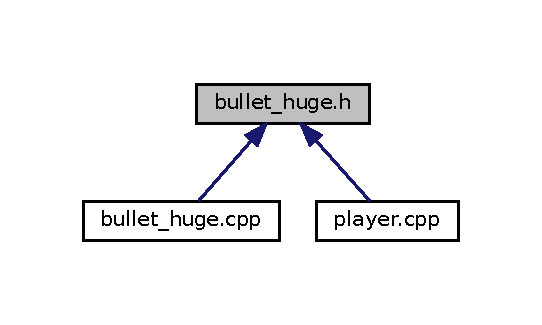
\includegraphics[width=260pt]{bullet__huge_8h__dep__incl}
\end{center}
\end{figure}
\subsection*{Classes}
\begin{DoxyCompactItemize}
\item 
class \hyperlink{classHugeBullet}{Huge\+Bullet}
\end{DoxyCompactItemize}

\hypertarget{colors_8cpp}{}\section{colors.\+cpp File Reference}
\label{colors_8cpp}\index{colors.\+cpp@{colors.\+cpp}}
{\ttfamily \#include \char`\"{}custom\+\_\+ncurses.\+h\char`\"{}}\newline
{\ttfamily \#include \char`\"{}colors.\+h\char`\"{}}\newline
Include dependency graph for colors.\+cpp\+:\nopagebreak
\begin{figure}[H]
\begin{center}
\leavevmode
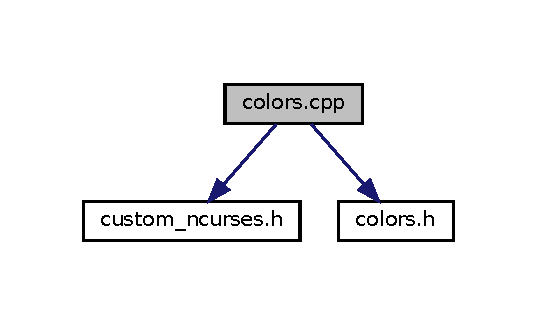
\includegraphics[width=258pt]{colors_8cpp__incl}
\end{center}
\end{figure}
\subsection*{Functions}
\begin{DoxyCompactItemize}
\item 
void \hyperlink{colors_8cpp_a188e9bf64f03d79aabbc6b049e6272d6}{init\+Pairs} ()
\begin{DoxyCompactList}\small\item\em Initialiases our custom color palette. \end{DoxyCompactList}\item 
void \hyperlink{colors_8cpp_a9f7a3915f1a267e6a625a7fcd0dc662e}{set\+Color} (\hyperlink{colors_8h_a37dbdc30935031c05304482e1be89d8f}{color} C\+O\+L\+OR)
\begin{DoxyCompactList}\small\item\em Sets current color used for all the drawing. \end{DoxyCompactList}\item 
void \hyperlink{colors_8cpp_a0f0ca5d3152f2107fbf03f79706225a4}{reset\+Color} (\hyperlink{colors_8h_a37dbdc30935031c05304482e1be89d8f}{color} C\+O\+L\+OR)
\begin{DoxyCompactList}\small\item\em Resets current color used for all the drawing. \end{DoxyCompactList}\end{DoxyCompactItemize}


\subsection{Function Documentation}
\mbox{\Hypertarget{colors_8cpp_a188e9bf64f03d79aabbc6b049e6272d6}\label{colors_8cpp_a188e9bf64f03d79aabbc6b049e6272d6}} 
\index{colors.\+cpp@{colors.\+cpp}!init\+Pairs@{init\+Pairs}}
\index{init\+Pairs@{init\+Pairs}!colors.\+cpp@{colors.\+cpp}}
\subsubsection{\texorpdfstring{init\+Pairs()}{initPairs()}}
{\footnotesize\ttfamily void init\+Pairs (\begin{DoxyParamCaption}{ }\end{DoxyParamCaption})}



Initialiases our custom color palette. 

$<$ Colors of player\textquotesingle{}s rocket

$<$ Colors of Huge\+Bullets power-\/up

$<$ Colors of Fast\+Bullets power-\/up

$<$ Colors of Triple\+Shot power-\/up

$<$ Colors of Classic\+Bullets power-\/down \mbox{\Hypertarget{colors_8cpp_a0f0ca5d3152f2107fbf03f79706225a4}\label{colors_8cpp_a0f0ca5d3152f2107fbf03f79706225a4}} 
\index{colors.\+cpp@{colors.\+cpp}!reset\+Color@{reset\+Color}}
\index{reset\+Color@{reset\+Color}!colors.\+cpp@{colors.\+cpp}}
\subsubsection{\texorpdfstring{reset\+Color()}{resetColor()}}
{\footnotesize\ttfamily void reset\+Color (\begin{DoxyParamCaption}\item[{\hyperlink{colors_8h_a37dbdc30935031c05304482e1be89d8f}{color}}]{C\+O\+L\+OR }\end{DoxyParamCaption})}



Resets current color used for all the drawing. 

\mbox{\Hypertarget{colors_8cpp_a9f7a3915f1a267e6a625a7fcd0dc662e}\label{colors_8cpp_a9f7a3915f1a267e6a625a7fcd0dc662e}} 
\index{colors.\+cpp@{colors.\+cpp}!set\+Color@{set\+Color}}
\index{set\+Color@{set\+Color}!colors.\+cpp@{colors.\+cpp}}
\subsubsection{\texorpdfstring{set\+Color()}{setColor()}}
{\footnotesize\ttfamily void set\+Color (\begin{DoxyParamCaption}\item[{\hyperlink{colors_8h_a37dbdc30935031c05304482e1be89d8f}{color}}]{C\+O\+L\+OR }\end{DoxyParamCaption})}



Sets current color used for all the drawing. 


\hypertarget{colors_8h}{}\section{colors.\+h File Reference}
\label{colors_8h}\index{colors.\+h@{colors.\+h}}
This graph shows which files directly or indirectly include this file\+:\nopagebreak
\begin{figure}[H]
\begin{center}
\leavevmode
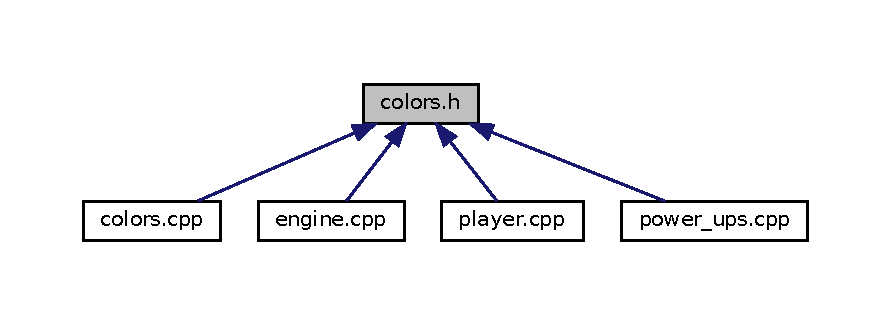
\includegraphics[width=350pt]{colors_8h__dep__incl}
\end{center}
\end{figure}
\subsection*{Enumerations}
\begin{DoxyCompactItemize}
\item 
enum \hyperlink{colors_8h_a37dbdc30935031c05304482e1be89d8f}{color} \{ \newline
\hyperlink{colors_8h_a37dbdc30935031c05304482e1be89d8fade5dc3e0dbd007d995ed3e37bde5ce7e}{P\+L\+A\+Y\+ER}, 
\hyperlink{colors_8h_a37dbdc30935031c05304482e1be89d8fa478a214d269ee52c13ff8f082bd9c28f}{H\+P\+O\+W\+ER}, 
\hyperlink{colors_8h_a37dbdc30935031c05304482e1be89d8fae5110cf2722db6f51453554e982e9a6e}{T\+P\+O\+W\+ER}, 
\hyperlink{colors_8h_a37dbdc30935031c05304482e1be89d8fafd8f2d571e0757949049642ef93bc38c}{C\+P\+O\+W\+ER}, 
\newline
\hyperlink{colors_8h_a37dbdc30935031c05304482e1be89d8fa2b29f78dc8cb3e3328def4aea33895bf}{F\+P\+O\+W\+ER}
 \}
\end{DoxyCompactItemize}
\subsection*{Functions}
\begin{DoxyCompactItemize}
\item 
void \hyperlink{colors_8h_a188e9bf64f03d79aabbc6b049e6272d6}{init\+Pairs} ()
\begin{DoxyCompactList}\small\item\em Initialiases our custom color palette. \end{DoxyCompactList}\item 
void \hyperlink{colors_8h_a9f7a3915f1a267e6a625a7fcd0dc662e}{set\+Color} (\hyperlink{colors_8h_a37dbdc30935031c05304482e1be89d8f}{color} C\+O\+L\+OR)
\begin{DoxyCompactList}\small\item\em Sets current color used for all the drawing. \end{DoxyCompactList}\item 
void \hyperlink{colors_8h_a0f0ca5d3152f2107fbf03f79706225a4}{reset\+Color} (\hyperlink{colors_8h_a37dbdc30935031c05304482e1be89d8f}{color} C\+O\+L\+OR)
\begin{DoxyCompactList}\small\item\em Resets current color used for all the drawing. \end{DoxyCompactList}\end{DoxyCompactItemize}


\subsection{Enumeration Type Documentation}
\mbox{\Hypertarget{colors_8h_a37dbdc30935031c05304482e1be89d8f}\label{colors_8h_a37dbdc30935031c05304482e1be89d8f}} 
\index{colors.\+h@{colors.\+h}!color@{color}}
\index{color@{color}!colors.\+h@{colors.\+h}}
\subsubsection{\texorpdfstring{color}{color}}
{\footnotesize\ttfamily enum \hyperlink{colors_8h_a37dbdc30935031c05304482e1be89d8f}{color}}

This header file contains helper functions to ease coloring of my custom sprites. \begin{DoxyEnumFields}{Enumerator}
\raisebox{\heightof{T}}[0pt][0pt]{\index{P\+L\+A\+Y\+ER@{P\+L\+A\+Y\+ER}!colors.\+h@{colors.\+h}}\index{colors.\+h@{colors.\+h}!P\+L\+A\+Y\+ER@{P\+L\+A\+Y\+ER}}}\mbox{\Hypertarget{colors_8h_a37dbdc30935031c05304482e1be89d8fade5dc3e0dbd007d995ed3e37bde5ce7e}\label{colors_8h_a37dbdc30935031c05304482e1be89d8fade5dc3e0dbd007d995ed3e37bde5ce7e}} 
P\+L\+A\+Y\+ER&\\
\hline

\raisebox{\heightof{T}}[0pt][0pt]{\index{H\+P\+O\+W\+ER@{H\+P\+O\+W\+ER}!colors.\+h@{colors.\+h}}\index{colors.\+h@{colors.\+h}!H\+P\+O\+W\+ER@{H\+P\+O\+W\+ER}}}\mbox{\Hypertarget{colors_8h_a37dbdc30935031c05304482e1be89d8fa478a214d269ee52c13ff8f082bd9c28f}\label{colors_8h_a37dbdc30935031c05304482e1be89d8fa478a214d269ee52c13ff8f082bd9c28f}} 
H\+P\+O\+W\+ER&\\
\hline

\raisebox{\heightof{T}}[0pt][0pt]{\index{T\+P\+O\+W\+ER@{T\+P\+O\+W\+ER}!colors.\+h@{colors.\+h}}\index{colors.\+h@{colors.\+h}!T\+P\+O\+W\+ER@{T\+P\+O\+W\+ER}}}\mbox{\Hypertarget{colors_8h_a37dbdc30935031c05304482e1be89d8fae5110cf2722db6f51453554e982e9a6e}\label{colors_8h_a37dbdc30935031c05304482e1be89d8fae5110cf2722db6f51453554e982e9a6e}} 
T\+P\+O\+W\+ER&\\
\hline

\raisebox{\heightof{T}}[0pt][0pt]{\index{C\+P\+O\+W\+ER@{C\+P\+O\+W\+ER}!colors.\+h@{colors.\+h}}\index{colors.\+h@{colors.\+h}!C\+P\+O\+W\+ER@{C\+P\+O\+W\+ER}}}\mbox{\Hypertarget{colors_8h_a37dbdc30935031c05304482e1be89d8fafd8f2d571e0757949049642ef93bc38c}\label{colors_8h_a37dbdc30935031c05304482e1be89d8fafd8f2d571e0757949049642ef93bc38c}} 
C\+P\+O\+W\+ER&\\
\hline

\raisebox{\heightof{T}}[0pt][0pt]{\index{F\+P\+O\+W\+ER@{F\+P\+O\+W\+ER}!colors.\+h@{colors.\+h}}\index{colors.\+h@{colors.\+h}!F\+P\+O\+W\+ER@{F\+P\+O\+W\+ER}}}\mbox{\Hypertarget{colors_8h_a37dbdc30935031c05304482e1be89d8fa2b29f78dc8cb3e3328def4aea33895bf}\label{colors_8h_a37dbdc30935031c05304482e1be89d8fa2b29f78dc8cb3e3328def4aea33895bf}} 
F\+P\+O\+W\+ER&\\
\hline

\end{DoxyEnumFields}


\subsection{Function Documentation}
\mbox{\Hypertarget{colors_8h_a188e9bf64f03d79aabbc6b049e6272d6}\label{colors_8h_a188e9bf64f03d79aabbc6b049e6272d6}} 
\index{colors.\+h@{colors.\+h}!init\+Pairs@{init\+Pairs}}
\index{init\+Pairs@{init\+Pairs}!colors.\+h@{colors.\+h}}
\subsubsection{\texorpdfstring{init\+Pairs()}{initPairs()}}
{\footnotesize\ttfamily void init\+Pairs (\begin{DoxyParamCaption}{ }\end{DoxyParamCaption})}



Initialiases our custom color palette. 

$<$ Colors of player\textquotesingle{}s rocket

$<$ Colors of Huge\+Bullets power-\/up

$<$ Colors of Fast\+Bullets power-\/up

$<$ Colors of Triple\+Shot power-\/up

$<$ Colors of Classic\+Bullets power-\/down \mbox{\Hypertarget{colors_8h_a0f0ca5d3152f2107fbf03f79706225a4}\label{colors_8h_a0f0ca5d3152f2107fbf03f79706225a4}} 
\index{colors.\+h@{colors.\+h}!reset\+Color@{reset\+Color}}
\index{reset\+Color@{reset\+Color}!colors.\+h@{colors.\+h}}
\subsubsection{\texorpdfstring{reset\+Color()}{resetColor()}}
{\footnotesize\ttfamily void reset\+Color (\begin{DoxyParamCaption}\item[{\hyperlink{colors_8h_a37dbdc30935031c05304482e1be89d8f}{color}}]{C\+O\+L\+OR }\end{DoxyParamCaption})}



Resets current color used for all the drawing. 

\mbox{\Hypertarget{colors_8h_a9f7a3915f1a267e6a625a7fcd0dc662e}\label{colors_8h_a9f7a3915f1a267e6a625a7fcd0dc662e}} 
\index{colors.\+h@{colors.\+h}!set\+Color@{set\+Color}}
\index{set\+Color@{set\+Color}!colors.\+h@{colors.\+h}}
\subsubsection{\texorpdfstring{set\+Color()}{setColor()}}
{\footnotesize\ttfamily void set\+Color (\begin{DoxyParamCaption}\item[{\hyperlink{colors_8h_a37dbdc30935031c05304482e1be89d8f}{color}}]{C\+O\+L\+OR }\end{DoxyParamCaption})}



Sets current color used for all the drawing. 


\hypertarget{custom__ncurses_8h}{}\section{custom\+\_\+ncurses.\+h File Reference}
\label{custom__ncurses_8h}\index{custom\+\_\+ncurses.\+h@{custom\+\_\+ncurses.\+h}}
This graph shows which files directly or indirectly include this file\+:
\nopagebreak
\begin{figure}[H]
\begin{center}
\leavevmode
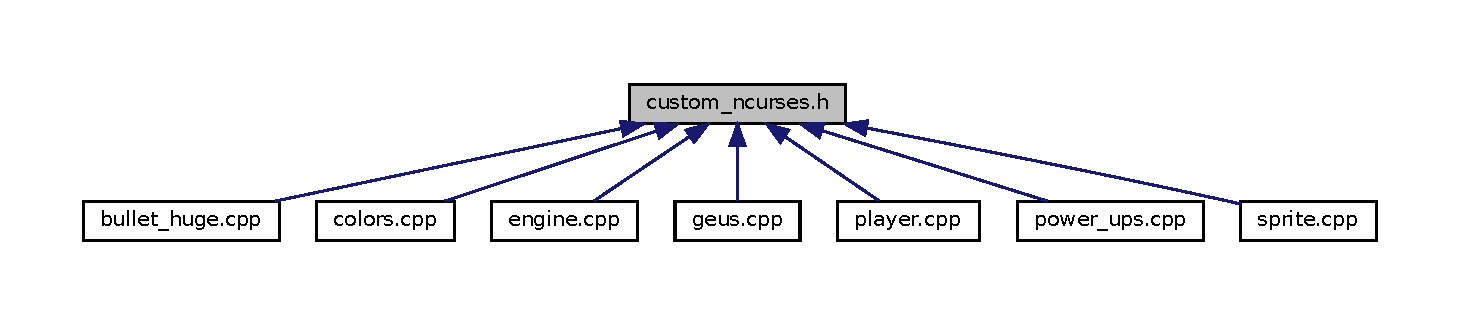
\includegraphics[width=350pt]{custom__ncurses_8h__dep__incl}
\end{center}
\end{figure}

\hypertarget{enemy_8cpp}{}\section{enemy.\+cpp File Reference}
\label{enemy_8cpp}\index{enemy.\+cpp@{enemy.\+cpp}}
{\ttfamily \#include \char`\"{}sprite.\+h\char`\"{}}\newline
{\ttfamily \#include \char`\"{}enemy.\+h\char`\"{}}\newline
Include dependency graph for enemy.\+cpp\+:
\nopagebreak
\begin{figure}[H]
\begin{center}
\leavevmode
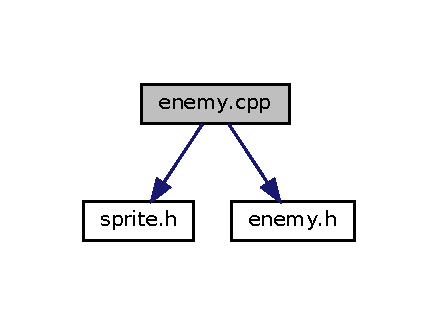
\includegraphics[width=210pt]{enemy_8cpp__incl}
\end{center}
\end{figure}

\hypertarget{enemy_8h}{}\section{enemy.\+h File Reference}
\label{enemy_8h}\index{enemy.\+h@{enemy.\+h}}
This graph shows which files directly or indirectly include this file\+:\nopagebreak
\begin{figure}[H]
\begin{center}
\leavevmode
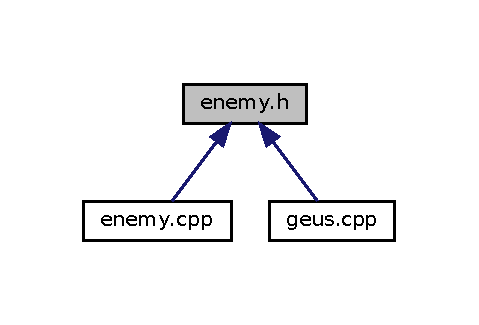
\includegraphics[width=230pt]{enemy_8h__dep__incl}
\end{center}
\end{figure}
\subsection*{Classes}
\begin{DoxyCompactItemize}
\item 
class \hyperlink{classEnemy}{Enemy}
\end{DoxyCompactItemize}

\hypertarget{engine_8cpp}{}\section{engine.\+cpp File Reference}
\label{engine_8cpp}\index{engine.\+cpp@{engine.\+cpp}}
{\ttfamily \#include \char`\"{}custom\+\_\+ncurses.\+h\char`\"{}}\newline
{\ttfamily \#include $<$thread$>$}\newline
{\ttfamily \#include \char`\"{}sprite.\+h\char`\"{}}\newline
{\ttfamily \#include \char`\"{}engine.\+h\char`\"{}}\newline
{\ttfamily \#include \char`\"{}colors.\+h\char`\"{}}\newline
Include dependency graph for engine.\+cpp\+:
\nopagebreak
\begin{figure}[H]
\begin{center}
\leavevmode
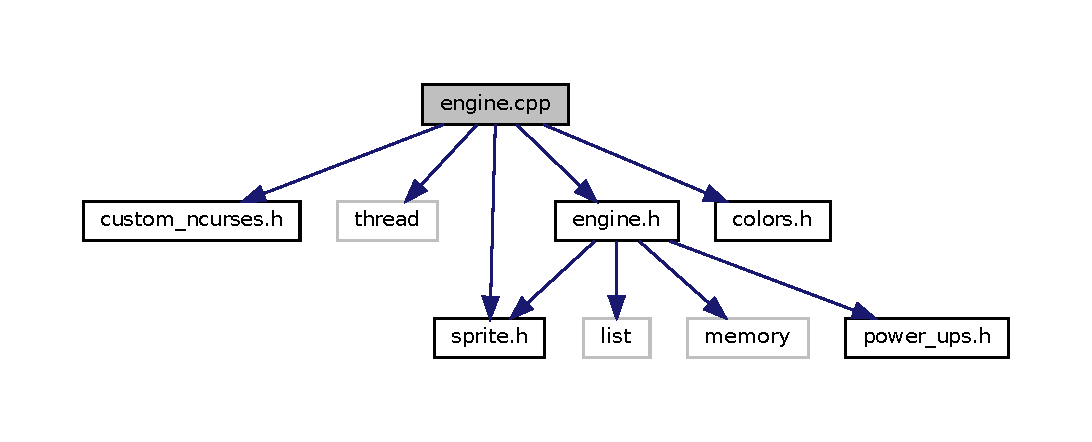
\includegraphics[width=350pt]{engine_8cpp__incl}
\end{center}
\end{figure}

\hypertarget{engine_8h}{}\section{engine.\+h File Reference}
\label{engine_8h}\index{engine.\+h@{engine.\+h}}
{\ttfamily \#include $<$list$>$}\newline
{\ttfamily \#include $<$memory$>$}\newline
{\ttfamily \#include \char`\"{}sprite.\+h\char`\"{}}\newline
{\ttfamily \#include \char`\"{}power\+\_\+ups.\+h\char`\"{}}\newline
Include dependency graph for engine.\+h\+:
\nopagebreak
\begin{figure}[H]
\begin{center}
\leavevmode
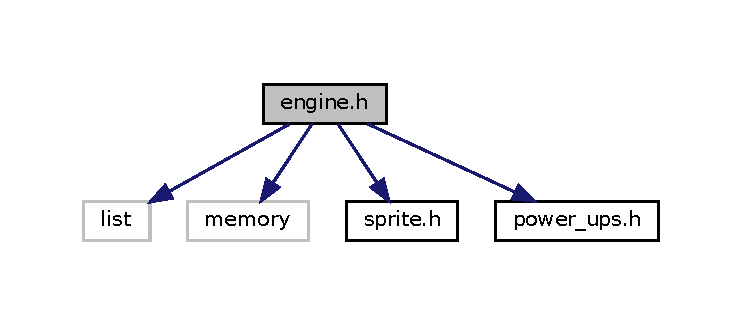
\includegraphics[width=350pt]{engine_8h__incl}
\end{center}
\end{figure}
This graph shows which files directly or indirectly include this file\+:
\nopagebreak
\begin{figure}[H]
\begin{center}
\leavevmode
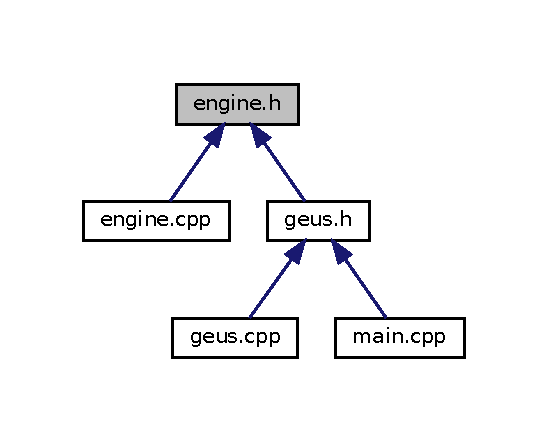
\includegraphics[width=263pt]{engine_8h__dep__incl}
\end{center}
\end{figure}
\subsection*{Classes}
\begin{DoxyCompactItemize}
\item 
class \hyperlink{classEngineWrapper}{Engine\+Wrapper}
\end{DoxyCompactItemize}

\hypertarget{geus_8cpp}{}\section{geus.\+cpp File Reference}
\label{geus_8cpp}\index{geus.\+cpp@{geus.\+cpp}}
{\ttfamily \#include \char`\"{}custom\+\_\+ncurses.\+h\char`\"{}}\newline
{\ttfamily \#include $<$fstream$>$}\newline
{\ttfamily \#include $<$cstring$>$}\newline
{\ttfamily \#include \char`\"{}geus.\+h\char`\"{}}\newline
{\ttfamily \#include \char`\"{}enemy.\+h\char`\"{}}\newline
Include dependency graph for geus.\+cpp\+:
\nopagebreak
\begin{figure}[H]
\begin{center}
\leavevmode
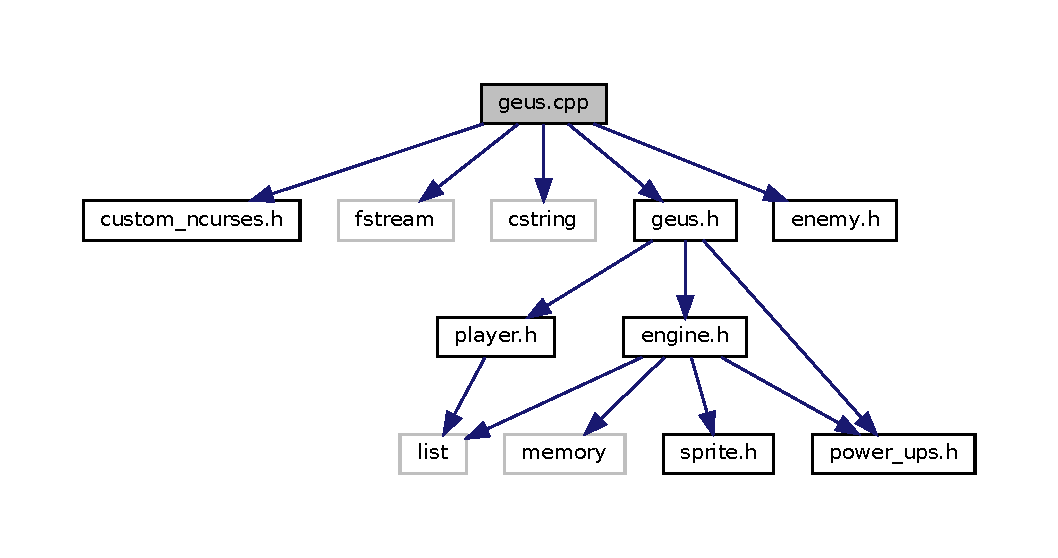
\includegraphics[width=350pt]{geus_8cpp__incl}
\end{center}
\end{figure}

\hypertarget{geus_8h}{}\section{geus.\+h File Reference}
\label{geus_8h}\index{geus.\+h@{geus.\+h}}
{\ttfamily \#include \char`\"{}engine.\+h\char`\"{}}\newline
{\ttfamily \#include \char`\"{}player.\+h\char`\"{}}\newline
{\ttfamily \#include \char`\"{}power\+\_\+ups.\+h\char`\"{}}\newline
Include dependency graph for geus.\+h\+:
\nopagebreak
\begin{figure}[H]
\begin{center}
\leavevmode
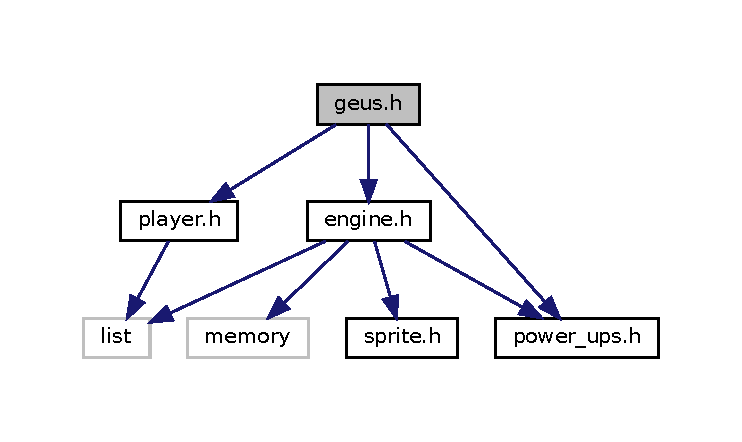
\includegraphics[width=350pt]{geus_8h__incl}
\end{center}
\end{figure}
This graph shows which files directly or indirectly include this file\+:
\nopagebreak
\begin{figure}[H]
\begin{center}
\leavevmode
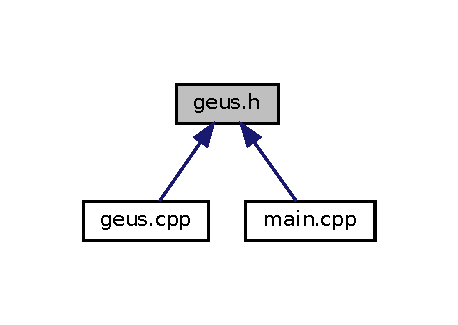
\includegraphics[width=220pt]{geus_8h__dep__incl}
\end{center}
\end{figure}
\subsection*{Classes}
\begin{DoxyCompactItemize}
\item 
class \hyperlink{classGeus}{Geus}
\end{DoxyCompactItemize}

\hypertarget{main_8cpp}{}\section{main.\+cpp File Reference}
\label{main_8cpp}\index{main.\+cpp@{main.\+cpp}}
{\ttfamily \#include $<$iostream$>$}\newline
{\ttfamily \#include \char`\"{}geus.\+h\char`\"{}}\newline
Include dependency graph for main.\+cpp\+:
\nopagebreak
\begin{figure}[H]
\begin{center}
\leavevmode
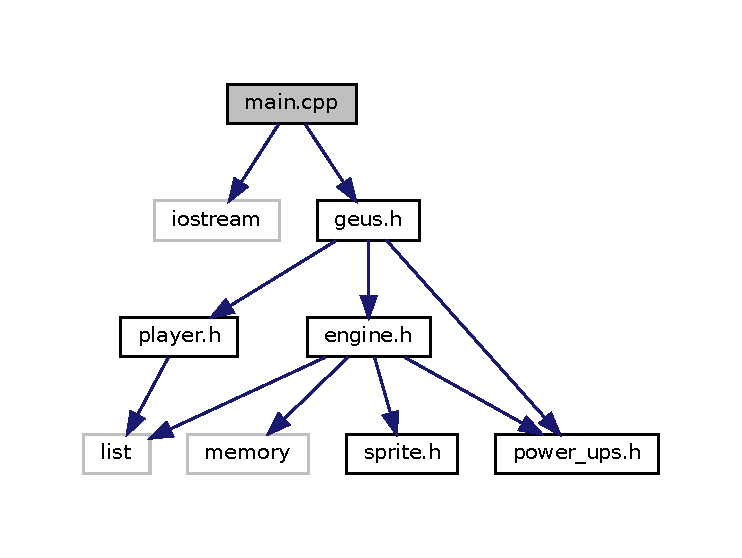
\includegraphics[width=350pt]{main_8cpp__incl}
\end{center}
\end{figure}
\subsection*{Functions}
\begin{DoxyCompactItemize}
\item 
int \hyperlink{main_8cpp_ae66f6b31b5ad750f1fe042a706a4e3d4}{main} ()
\end{DoxyCompactItemize}


\subsection{Function Documentation}
\mbox{\Hypertarget{main_8cpp_ae66f6b31b5ad750f1fe042a706a4e3d4}\label{main_8cpp_ae66f6b31b5ad750f1fe042a706a4e3d4}} 
\index{main.\+cpp@{main.\+cpp}!main@{main}}
\index{main@{main}!main.\+cpp@{main.\+cpp}}
\subsubsection{\texorpdfstring{main()}{main()}}
{\footnotesize\ttfamily int main (\begin{DoxyParamCaption}{ }\end{DoxyParamCaption})}


\hypertarget{player_8cpp}{}\section{player.\+cpp File Reference}
\label{player_8cpp}\index{player.\+cpp@{player.\+cpp}}
{\ttfamily \#include \char`\"{}custom\+\_\+ncurses.\+h\char`\"{}}\newline
{\ttfamily \#include $<$cmath$>$}\newline
{\ttfamily \#include \char`\"{}sprite.\+h\char`\"{}}\newline
{\ttfamily \#include \char`\"{}player.\+h\char`\"{}}\newline
{\ttfamily \#include \char`\"{}colors.\+h\char`\"{}}\newline
{\ttfamily \#include \char`\"{}bullet.\+h\char`\"{}}\newline
{\ttfamily \#include \char`\"{}bullet\+\_\+huge.\+h\char`\"{}}\newline
{\ttfamily \#include \char`\"{}bullet\+\_\+fast.\+h\char`\"{}}\newline
Include dependency graph for player.\+cpp\+:\nopagebreak
\begin{figure}[H]
\begin{center}
\leavevmode
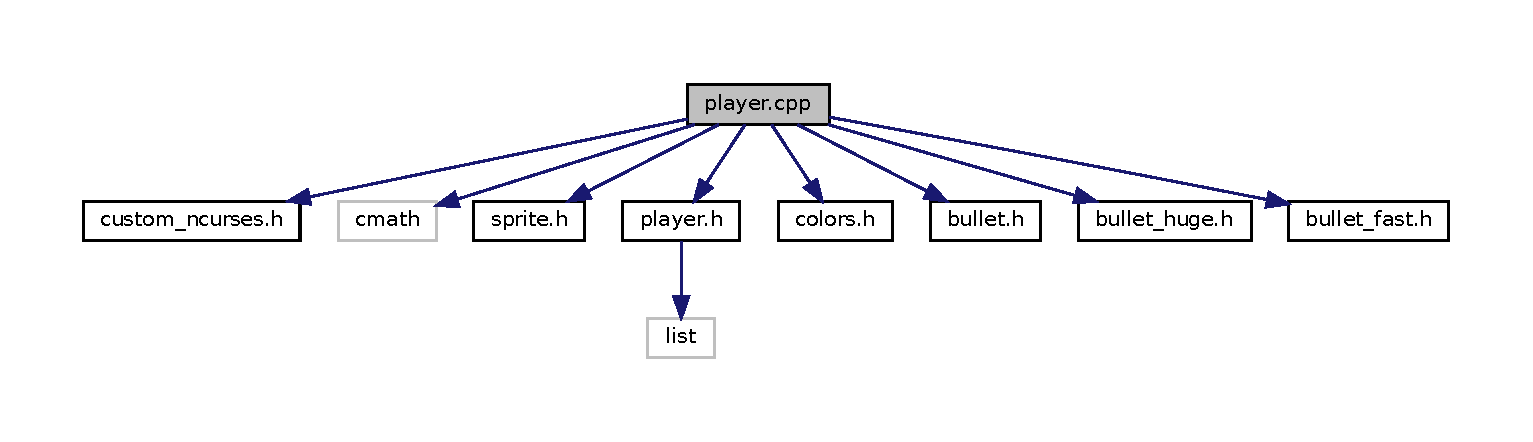
\includegraphics[width=350pt]{player_8cpp__incl}
\end{center}
\end{figure}

\hypertarget{player_8h}{}\section{player.\+h File Reference}
\label{player_8h}\index{player.\+h@{player.\+h}}
{\ttfamily \#include $<$list$>$}\newline
Include dependency graph for player.\+h\+:
\nopagebreak
\begin{figure}[H]
\begin{center}
\leavevmode
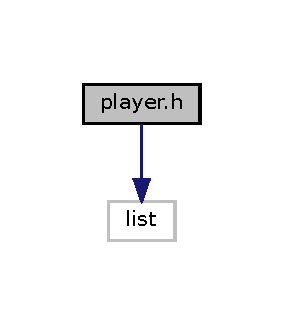
\includegraphics[width=136pt]{player_8h__incl}
\end{center}
\end{figure}
This graph shows which files directly or indirectly include this file\+:
\nopagebreak
\begin{figure}[H]
\begin{center}
\leavevmode
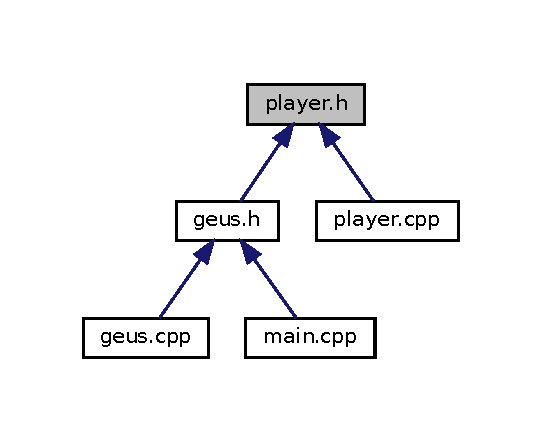
\includegraphics[width=260pt]{player_8h__dep__incl}
\end{center}
\end{figure}
\subsection*{Classes}
\begin{DoxyCompactItemize}
\item 
class \hyperlink{classPlayer}{Player}
\end{DoxyCompactItemize}

\hypertarget{power__ups_8cpp}{}\section{power\+\_\+ups.\+cpp File Reference}
\label{power__ups_8cpp}\index{power\+\_\+ups.\+cpp@{power\+\_\+ups.\+cpp}}
{\ttfamily \#include \char`\"{}custom\+\_\+ncurses.\+h\char`\"{}}\newline
{\ttfamily \#include \char`\"{}sprite.\+h\char`\"{}}\newline
{\ttfamily \#include \char`\"{}power\+\_\+ups.\+h\char`\"{}}\newline
{\ttfamily \#include \char`\"{}colors.\+h\char`\"{}}\newline
Include dependency graph for power\+\_\+ups.\+cpp\+:\nopagebreak
\begin{figure}[H]
\begin{center}
\leavevmode
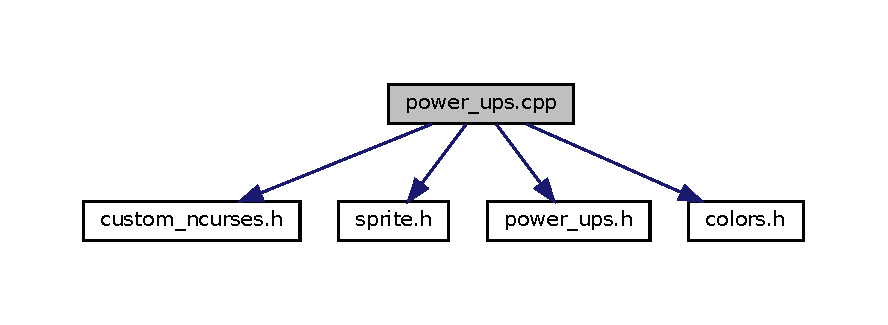
\includegraphics[width=350pt]{power__ups_8cpp__incl}
\end{center}
\end{figure}

\hypertarget{power__ups_8h}{}\section{power\+\_\+ups.\+h File Reference}
\label{power__ups_8h}\index{power\+\_\+ups.\+h@{power\+\_\+ups.\+h}}
This graph shows which files directly or indirectly include this file\+:
\nopagebreak
\begin{figure}[H]
\begin{center}
\leavevmode
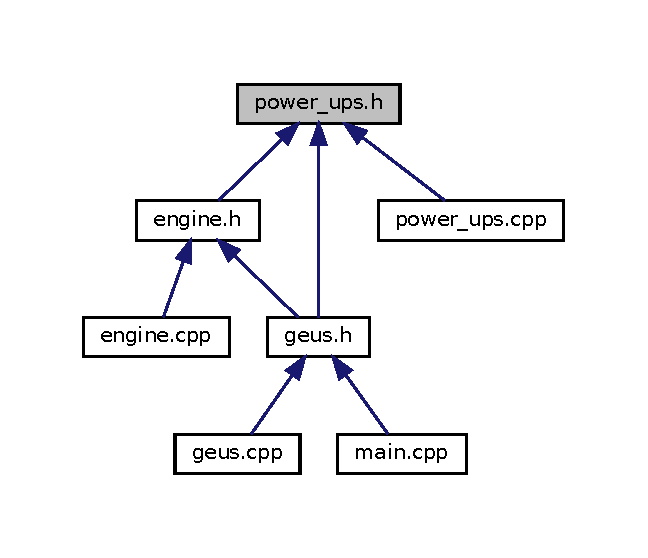
\includegraphics[width=311pt]{power__ups_8h__dep__incl}
\end{center}
\end{figure}
\subsection*{Classes}
\begin{DoxyCompactItemize}
\item 
class \hyperlink{classCPowerUp}{C\+Power\+Up}
\item 
class \hyperlink{classTriPowerUp}{Tri\+Power\+Up}
\item 
class \hyperlink{classHBPowerUp}{H\+B\+Power\+Up}
\item 
class \hyperlink{classFPowerUp}{F\+Power\+Up}
\end{DoxyCompactItemize}

\hypertarget{README_8md}{}\section{R\+E\+A\+D\+M\+E.\+md File Reference}
\label{README_8md}\index{R\+E\+A\+D\+M\+E.\+md@{R\+E\+A\+D\+M\+E.\+md}}

\hypertarget{sprite_8cpp}{}\section{sprite.\+cpp File Reference}
\label{sprite_8cpp}\index{sprite.\+cpp@{sprite.\+cpp}}
{\ttfamily \#include \char`\"{}custom\+\_\+ncurses.\+h\char`\"{}}\newline
{\ttfamily \#include \char`\"{}sprite.\+h\char`\"{}}\newline
Include dependency graph for sprite.\+cpp\+:\nopagebreak
\begin{figure}[H]
\begin{center}
\leavevmode
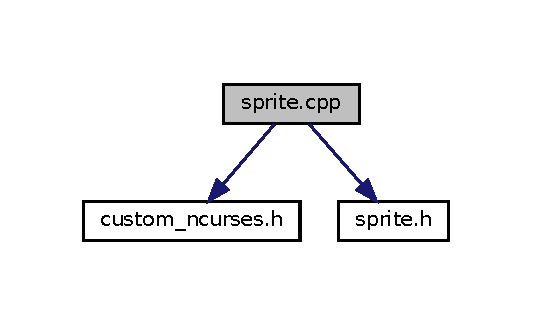
\includegraphics[width=256pt]{sprite_8cpp__incl}
\end{center}
\end{figure}

\hypertarget{sprite_8h}{}\section{sprite.\+h File Reference}
\label{sprite_8h}\index{sprite.\+h@{sprite.\+h}}
This graph shows which files directly or indirectly include this file\+:\nopagebreak
\begin{figure}[H]
\begin{center}
\leavevmode
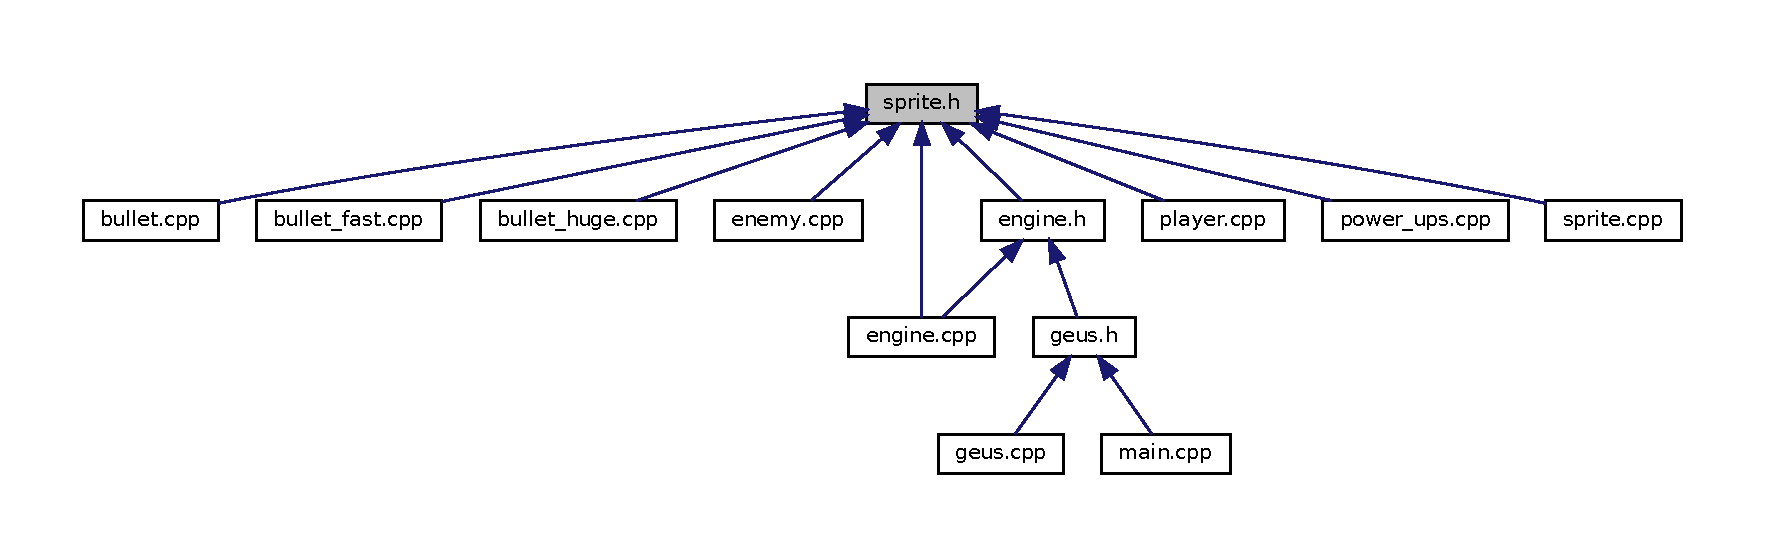
\includegraphics[width=350pt]{sprite_8h__dep__incl}
\end{center}
\end{figure}
\subsection*{Classes}
\begin{DoxyCompactItemize}
\item 
class \hyperlink{classSprite}{Sprite}
\end{DoxyCompactItemize}

%--- End generated contents ---

% Index
\backmatter
\newpage
\phantomsection
\clearemptydoublepage
\addcontentsline{toc}{chapter}{Index}
\printindex

\end{document}
